%! TeX program = lualatex

% NOTE: Use twoside for the final print and oneside for the digital version
\documentclass[a4paper,oneside,12pt]{report}
\usepackage[italian]{babel}
\usepackage{graphicx}
\usepackage{tikz}
\usetikzlibrary{positioning}
\usepackage{hyphenat}
\hyphenation{mate-mati-ca recu-perare}
\usepackage{hyperref}
\hypersetup{
	colorlinks=true,
	allcolors=black
}
\usepackage{parskip}

\usepackage{tocloft}
\renewcommand{\cftchapdotsep}{\cftdotsep}

\linespread{1.25}

\makeatletter
\def\cleardoublepage{\clearpage\if@twoside \ifodd\c@page\else
	\hbox{}
	\vspace*{\fill}
	\vspace{\fill}
	\thispagestyle{empty}
	\newpage
	\if@twocolumn\hbox{}\newpage\fi\fi\fi}
\makeatother

\begin{document}
	\begin{titlepage}
		\begin{tikzpicture}[remember picture,overlay]
			\centering
			\node[yshift=-6 cm] (logo) at (current page.north) {
\includegraphics[width=0.75\linewidth]{figures/uniba.jpg}};
			\node[text width=50em,yshift=0.25cm, align = center, below = of logo](dipartimento){\normalsize {Dipartimento di Informatica}};
			\node[text width=40em, align = center, yshift=.55cm,below = of dipartimento](course){\normalsize {Corso di Laurea in Informatica}};
			\node[text width=35em,align = center,  yshift=1.2cm,below = of course](line){\par\noindent\rule{\textwidth}{0.4pt}};
			\node[text width=40em, align = center, yshift=.55cm,below = of line](lia){\normalsize {Tesi di Laurea \\ in \\ Linguaggi di Programmazione}};

			\node[text width=40em, align = center, yshift=-0.5cm,below = of lia](title){\parbox{12cm}{\centering {\bfseries \fontsize{20pt}{20pt}\selectfont {BugginOut}} \\ \vspace{0.5cm} {\fontsize{16pt}{16pt}\selectfont {Design e implementazione di un linguaggo di programmazione}}\par}};

			\node[text width=35em, align = left, yshift=-1cm,below = of title](relatoretit){\normalsize \textbf{Relatore} };
			\node[text width=35em, align = left, yshift=1cm,below = of relatoretit](relatore){\large {Prof. Pasquale Lops}};

			\node[text width=35em, align = right, yshift=-1cm,below = of title](candidatetit){\normalsize \textbf{Laureando}};
			\node[text width=35em, align = right, yshift=1cm,below = of candidatetit](candidate){\large {Davide Carella}};

			\node[text width=35em,align = center,  yshift= -3cm,below = of candidate](line2){\par\noindent\rule{\textwidth}{0.4pt}};
			\node[text width=50em, align = center, yshift=0.5cm,below = of line2](year){\large {Anno accademico: 2024 - 2025}};
		\end{tikzpicture}
	\end{titlepage}

	\pagenumbering{roman}

	\cleardoublepage
	\addcontentsline{toc}{chapter}{Abstract}
	% LTeX: language=it

\chapter*{Abstract}

Questo elaborato presenta \textit{BugginOut}, un linguaggio di programmazione moderno e minimale progettato per essere espressivo e accessibile. Dopo una panoramica sulle scelte di design si procede con la descrizione del flusso di compilazione nelle sue fasi principali: analisi lessicale, grammaticale e semantica, fino alla generazione del codice. L'architettura del compilatore viene poi analizzata nel dettaglio, seguita da una selezione di programmi di esempio che dimostrano le potenzialità del linguaggio. In chiusura, si discutono gli attuali limiti e possibili sviluppi futuri del linguaggio con alcune riflessioni finali.

	\cleardoublepage
	\addcontentsline{toc}{chapter}{Indice}
	\tableofcontents
	\cleardoublepage

	\pagenumbering{arabic}
	\setcounter{page}{1}

	\addcontentsline{toc}{chapter}{Introduzione}
	% LTeX: language=it

\chapter*{Introduzione}
\label{chap:introduzione}

BugginOut \`e un linguaggio di programmazione \textit{general-purpose} transpilato in C++ e sviluppato in C++ da zero. Il progetto nasce dall'analisi di linguaggi esistenti, dai quali sono state reinterpretate le funzionalit\`a ritenute pi\`u efficaci, con l'obiettivo di creare un linguaggio nuovo sintatticamente semplice, moderno e leggibile.

Il nome BugginOut \`e un gioco di parole sul termine \textit{bug} e il personaggio omonimo \textit{Buggin' Out} del film \textit{Do The Right Thing} di Spike Lee. Questo, oltre a essere un omaggio al film, rappresenta anche il concetto di \textit{debugging} e la ricerca di un linguaggio che possa aiutare i programmatori a scrivere codice pi\`u facilmente e senza errori.

Nel capitolo \ref{chap:flusso-di-compilazione} si analizzano tutte le fasi che portano un programma scritto in BugginOut (solitamente un file con estensione \texttt{.bo}), in particolare:
\begin{itemize}
	\item nel paragrafo \ref{sec:analisi-lessicale} si esamina la prima fase di compilazione: l'analisi lessicale del codice che consiste nella trasformazione del programma (un insieme di caratteri) in un insieme di \emph{token} (la parte atomica di ogni programma);
	\item nel paragrafo \ref{sec:analisi-grammaticale} si esamina l'analisi grammaticale del codice: la trasformazione dell'insieme di \emph{token} prodotto dall'analisi lessicale in un \emph{AST} (\textit{Abstract Syntax Tree}), un albero che rappresenta la struttura di un programma (o una sua parte) senza, per\`o, le informazioni contestuali;
	\item nel paragrafo \ref{sec:analisi-semantica} si esamina l'analisi semantica del codice: l'arricchimento dell'AST generato dall'analisi grammaticale viene con informazioni contestuali come, ad esempio, variabili e funzioni dichiarate e i tipi utilizzati nel programma;
	\item nel paragrafo \ref{sec:generazione-del-codice} si esamina la fase finale della compilazione: la generazione del codice C++ finale che viene poi compilato, da un compilatore C++ gi\`a esistente, nell'eseguibile finale del programma.
\end{itemize}
Nel capitolo \ref{chap:architettura-del-compilatore} si analizzano nel dettaglio le astrazioni utilizzate per realizzare il compilatore, tra cui:
\begin{itemize}
	\item il \texttt{Lexer} genera dei \texttt{Token} su richiesta a partire da un programma;
	\item il \texttt{Parser} genera un'\texttt{AST} ovvero una gerarchia di \texttt{Node}, la classe madre di ogni nodo dell'albero;
	\item il \texttt{Typechecker} controlla il corretto utilizzo di tipi, variabili e funzioni nel programma per poi generare un \texttt{CheckedAST};
	\item il \texttt{Transpiler} trasforma il \texttt{CheckedAST} nel codice C++ finale.
\end{itemize}
Le astrazioni introdotte in questo capitolo trovano una corrispondenza uno-a-uno con le fasi del flusso di compilazione descritte nel capitolo \ref{chap:flusso-di-compilazione}, poiché esse rappresentano l’implementazione concreta di ciascuna di tali fasi.

Nel capitolo \ref{chap:design-del-linguaggio} vengono delineate le scelte progettuali del linguaggio, in particolare se ne analizzer\`a i tipi di dato disponibili e la sintassi.

Nel capitolo \ref{chap:alcuni-esempi} si analizzano alcuni algoritmi implementati in BugginOut per dimostrarne l'espressivit\`a e, infine, si conclude esaminando i limiti del linguaggio allo stato attuale, i possibili sviluppi futuri e si giunge a una valutazione complessiva del lavoro svolto.

	\chapter{Design del linguaggio}

\section{Sintassi}

\section{Tipi di dato}

\section{Control flow}

	% LTeX: language=it

\chapter{Flusso di compilazione}
\label{chap:flusso-di-compilazione}

Nel seguente capitolo si affronteranno, separatamente, le fasi di compilazione di un programma scritto in BugginOut. \`E bene notare che ciascuna di queste fasi prende in ingresso il risultato della fase precedente.

\section{Analisi lessicale}
\label{sec:analisi-lessicale}

Da \cite{alfred2007compilers}:
\begin{parcolumns}[colwidths={1=0.44\textwidth,2=0.44\textwidth},rulebetween=true,nofirstindent=true,sloppy=true]{2}
	% LTeX: language=en_us
	\colchunk{
		\leftskip=1em
		``The main task of the lexical analyzer is to read the input characters of the \emph{source} program, group them into \emph{lexemes}, and produce as output a sequence of \emph{tokens} for each lexeme in the source program.

		[\ldots]

		When discussing lexical analysis, we use three related but distinct terms:
		\begin{itemize}
			\item A \emph{token} is a pair consisting of a token \emph{name} and an optional attribute \emph{value}. The token name is an abstract symbol representing a kind of lexical unit, e.g., a particular keyword, or a sequence of input characters denoting an identifier. [\ldots]
			\item A \emph{pattern} is a description of the form that the lexemes of a token may take. In the case of a kewyord as a token, the pattern is just the sequence of characters that form the keyword. For identifiers and some other tokens, the pattern is a more complex structure that is matched by many strings.
			\item A \emph{lexeme} is a sequence of characters in the source program that matches the pattern for a token and is identified by the lexical analyzer as an instance of that token.''
		\end{itemize}
	}
	% LTeX: language=it
	\colchunk{
		\leftskip=1em
		``Il compito principale di un analizzatore lessicale \`e la lettura dei caratteri di input del programma \emph{sorgente}, raggrupparli in \emph{lessemi} e produrre, come risultato, una sequenza di \emph{token} per ogni lessema del programma sorgente.

		[\ldots]

		Durante la discussione dell'analisi lessicale, si usano tre legati ma distinti termini:
		\begin{itemize}
			\item Un \emph{token} \`e una coppia costituita di un \emph{nome} e un \emph{valore} opzionale. Il nome \`e un simbolo astratto che rappresenta il tipo di unit\`a lessicale, ad esempio, una particolare parola chiave oppure una sequenza di caratteri che denota un identificatore. [\dots]
			\item Un \emph{pattern} \`e una descrizione della forma che i lessemi di un token possono avere. Nel caso di una parola chiave come token, il pattern \`e semplicemente la sequenza di caratteri che formano la parola chiave. Per gli identificatori e qualche altro token, il pattern \`e una struttura pi\`u complessa che riconosce pi\`u stringhe.
			\item Un \emph{lessema} \`e una sequenza di caratteri del programma sorgente.''
		\end{itemize}
	}
	\colplacechunks
\end{parcolumns}

\begin{table}[H]
	\begin{tabularx}{\textwidth}{X|X|X}
		\hline
		\hline
		\multicolumn{1}{c|}{\textsc{Token}} & \multicolumn{1}{c|}{\textsc{Pattern} (informale)} & \multicolumn{1}{c}{\textsc{Lessemi}} \\
		\hline
		\texttt{kw\_for} & i seguenti caratteri: \texttt{for} & \texttt{for} \\
		\hline
		\texttt{kw\_if} & i seguenti caratteri: \texttt{if} & \texttt{if} \\
		\hline
		\texttt{Identifier} & una lettera oppure \mbox{\texttt{\_} o \texttt{\$}} seguita da una serie di lettere, cifre numeriche oppure \mbox{\texttt{\_} o \texttt{\$}} & \texttt{a}, \texttt{b}, \texttt{token\_name}, \texttt{num1}, \ldots \\
		\hline
		\texttt{IntegerLiteral} & uno o pi\`u cifre decimali\footnotemark & \texttt{1}, \texttt{123}, \ldots \\
		\hline
		\hline
	\end{tabularx}
	\caption{Alcuni token di BugginOut}
	\label{fig:bugginout-example-tokens}
\end{table}

\footnotetext{In BugginOut \`e possibile utilizzare i numeri in notazione binari, ottale ed esadecimale. Per esempio \texttt{0b101} \`e un numero binario, \texttt{0o127} \`e un numero ottale e \texttt{0x1A} \`e un numero esadecimale. Inoltre possono essere seguiti da un suffisso per indicarne il tipo. Il pattern per entrambi \`e stato omesso in quanto non rilevante per l'esempio.}

Nella fase di analisi lessicale si alternano due operazioni:
\begin{itemize}
	\item definita da \cite{alfred2007compilers} come \emph{scanning}, si ignorano i caratteri che non sono significativi per il linguaggio (spazi bianchi e \emph{commenti});
	\item definita da \cite{alfred2007compilers} come \emph{lexical analysis}, \`e la parte pi\`u complessa in cui si producono i token.
\end{itemize}

Quando pi\`u di un lessema pu\`o essere riconosciuto da un pattern, l'analizzatore lessicale inserisce nel valore delle informazioni aggiuntive utili alle fasi successive di compilazione. Ad esempio, nel caso di un numero, il valore \`e il numero stesso. Ad esempio, facendo riferimento all'esempio \ref{fig:bugginout-example-tokens}, il token \texttt{IntegerLiteral} conterrebbe come valore \texttt{123}.

\`E importante osservare che ci\`o che influenzer\`a le decisioni di analisi grammaticale del compilatore \`e il nome del token e non il suo valore che, invece, viene usato per la traduzione dei token.

Per completezza, di seguito verranno riportati tutti i token definiti in BugginOut.
\begin{xltabular}{\textwidth}{l|X}
	\caption{Token di BugginOut}
	\label{fig:bugginout-complete-tokens} \\

	\hline
	\hline
	\multicolumn{1}{c|}{\textsc{Token}} & \multicolumn{1}{c|}{\textsc{Pattern} (in POSIX ERE \cite{iso-9945-2009})} \\
	\hline
	\endfirsthead

	\hline
	\multicolumn{1}{c|}{\textsc{Token}} & \multicolumn{1}{c|}{\textsc{Pattern}} \\
	\hline
	\endhead

	\endfoot

	\hline
	\hline
	\endlastfoot

	\texttt{kw\_anon} & \texttt{anon} \\ \hline
	\texttt{kw\_as} & \texttt{as} \\ \hline
	\texttt{kw\_bool} & \texttt{bool} \\ \hline
	\texttt{kw\_break} & \texttt{break} \\ \hline
	\texttt{kw\_char} & \texttt{char} \\ \hline
	\texttt{kw\_continue} & \texttt{continue} \\ \hline
	\texttt{kw\_else} & \texttt{else} \\ \hline
	\texttt{kw\_f32} & \texttt{f32} \\ \hline
	\texttt{kw\_f64} & \texttt{f64} \\ \hline
	\texttt{kw\_false} & \texttt{false} \\ \hline
	\texttt{kw\_fn} & \texttt{fn} \\ \hline
	\texttt{kw\_for} & \texttt{for} \\ \hline
	\texttt{kw\_i16} & \texttt{i16} \\ \hline
	\texttt{kw\_i32} & \texttt{i32} \\ \hline
	\texttt{kw\_i64} & \texttt{i64} \\ \hline
	\texttt{kw\_i8} & \texttt{i8} \\ \hline
	\texttt{kw\_if} & \texttt{if} \\ \hline
	\texttt{kw\_in} & \texttt{in} \\ \hline
	\texttt{kw\_isize} & \texttt{isize} \\ \hline
	\texttt{kw\_mut} & \texttt{mut} \\ \hline
	\texttt{kw\_null} & \texttt{null} \\ \hline
	\texttt{kw\_return} & \texttt{return} \\ \hline
	\texttt{kw\_true} & \texttt{true} \\ \hline
	\texttt{kw\_u16} & \texttt{u16} \\ \hline
	\texttt{kw\_u32} & \texttt{u32} \\ \hline
	\texttt{kw\_u64} & \texttt{u64} \\ \hline
	\texttt{kw\_u8} & \texttt{u8} \\ \hline
	\texttt{kw\_usize} & \texttt{usize} \\ \hline
	\texttt{kw\_var} & \texttt{var} \\ \hline
	\texttt{kw\_void} & \texttt{void} \\ \hline
	\texttt{Ampersand} & \texttt{\&} \\ \hline
	\texttt{AmpersandEquals} & \texttt{\&=} \\ \hline
	\texttt{Asterisk} & \texttt{*} \\ \hline
	\texttt{AsteriskEquals} & \texttt{*=} \\ \hline
	\texttt{At} & \texttt{@} \\ \hline
	\texttt{BinaryLiteral} & \texttt{0b[01]+(\_[a-zA-Z\_\$][a-zA-Z\_\$0-9]*)?}  \\ \hline
	\texttt{CharLiteral} & \texttt{\textquotesingle([\textasciicircum \textquotesingle \textbackslash \textbackslash]|\textbackslash \textbackslash \textquotesingle |\textbackslash \textbackslash n|\textbackslash \textbackslash r|\textbackslash \textbackslash t|\textbackslash\textbackslash\textbackslash\textbackslash|\textbackslash \textbackslash 0|\textbackslash \textbackslash x[0-7][0-9a-fA-F])\textquotesingle} \\ \hline
	\texttt{Circumflex} & \texttt{\textbackslash\textasciicircum} \\ \hline
	\texttt{CircumflexEquals} & \texttt{\textbackslash\textasciicircum=} \\ \hline
	\texttt{Colon} & \texttt{:} \\ \hline
	\texttt{Comma} & \texttt{,} \\ \hline
	\texttt{DecimalLiteral} & \texttt{[0-9]+(\_[a-zA-Z\_\$][a-zA-Z\_\$0-9]*)?} \\ \hline
	\texttt{Dot} & \texttt{\textbackslash .} \\ \hline
	\texttt{DotDotEquals} & \texttt{\textbackslash .\textbackslash .=} \\ \hline
	\texttt{DotDotLessThan} & \texttt{\textbackslash .\textbackslash .<} \\ \hline
	\texttt{DoubleAmpersand} & \texttt{\&\&} \\ \hline
	\texttt{DoubleAmpersandEquals} & \texttt{\&\&=} \\ \hline
	\texttt{DoubleEquals} & \texttt{==} \\ \hline
	\texttt{DoublePipe} & \texttt{\textbackslash |\textbackslash |} \\ \hline
	\texttt{DoublePipeEquals} & \texttt{\textbackslash |\textbackslash |=} \\ \hline
	\texttt{EndOfFile} & Non ha un pattern associato in quanto viene generato quando l'analizzatore lessicale ha terminato di analizzare il programma sorgente. \\ \hline
	\texttt{Equals} & \texttt{=} \\ \hline
	\texttt{ExclamationMark} & \texttt{!} \\ \hline
	\texttt{ExclamationMarkEquals} & \texttt{!=} \\ \hline
	\texttt{FloatLiteral} & \texttt{[0-9]+\textbackslash.[0-9]+(\_[a-zA-Z\_\$][a-zA-Z\_\$0-9]*)?} \\ \hline
	\texttt{GreaterThan} & \texttt{>} \\ \hline
	\texttt{GreaterThanEquals} & \texttt{>=} \\ \hline
	\texttt{HexadecimalLiteral} & \texttt{0x[0-9a-fA-F]+(\_[a-zA-Z\_\$][a-zA-Z\_\$0-9]*)?} \\ \hline
	\texttt{Identifier} & \texttt{[a-zA-Z\_\$][a-zA-Z\_\$0-9]*} \\ \hline
	\texttt{LeftCurlyBracket} & \texttt{\{} \\ \hline
	\texttt{LeftParenthesis} & \texttt{\textbackslash (} \\ \hline
	\texttt{LeftShift} & \texttt{<<} \\ \hline
	\texttt{LeftShiftEquals} & \texttt{<<=} \\ \hline
	\texttt{LeftSquareBracket} & \texttt{\textbackslash \char"5B} \\ \hline
	\texttt{LessThan} & \texttt{<} \\ \hline
	\texttt{LessThanEquals} & \texttt{<=} \\ \hline
	\texttt{Minus} & \texttt{-} \\ \hline
	\texttt{MinusEquals} & \texttt{-=} \\ \hline
	\texttt{MinusMinus} & \texttt{--} \\ \hline
	\texttt{OctalLiteral} & \texttt{0o[0-7]+(\_[a-zA-Z\_\$][a-zA-Z\_\$0-9]*)?} \\ \hline
	\texttt{Percent} & \texttt{\%} \\ \hline
	\texttt{PercentEquals} & \texttt{\%=} \\ \hline
	\texttt{Pipe} & \texttt{\textbackslash |} \\ \hline
	\texttt{PipeEquals} & \texttt{\textbackslash |=} \\ \hline
	\texttt{Plus} & \texttt{+} \\ \hline
	\texttt{PlusEquals} & \texttt{+=} \\ \hline
	\texttt{PlusPlus} & \texttt{++} \\ \hline
	\texttt{RightCurlyBracket} & \texttt{\}} \\ \hline
	\texttt{RightParenthesis} & \texttt{\textbackslash )} \\ \hline
	\texttt{RightShift} & \texttt{>>} \\ \hline
	\texttt{RightShiftEquals} & \texttt{>>=} \\ \hline
	\texttt{RightSquareBracket} & \texttt{\textbackslash ]} \\ \hline
	\texttt{Semicolon} & \texttt{;} \\ \hline
	\texttt{Solidus} & \texttt{/} \\ \hline
	\texttt{SolidusEquals} & \texttt{/=} \\ \hline
	\texttt{StringLiteral} & \texttt{\textquotedbl ([\textasciicircum \textquotedbl \textbackslash \textbackslash]|\textbackslash \textbackslash \textquotedbl|\textbackslash \textbackslash n|\textbackslash \textbackslash r|\textbackslash \textbackslash t|\textbackslash \textbackslash \textbackslash \textbackslash|\textbackslash \textbackslash 0|\textbackslash \textbackslash x[0-7][0-9a-fA-F])*\textquotedbl} \\ \hline
	\texttt{Tilde} & \texttt{\textasciitilde}
\end{xltabular}
Per riconoscere i token, si passa dai pattern ad una rappresentazione intermedia: i \textit{transition diagram}. Questi vengono definiti da \cite{alfred2007compilers} e non sono altro che degli automi a stati finiti.
\begin{figure}[H]
	\centering
	\begin{tikzpicture}[node distance=3.5cm, on grid, auto]
		\node[state, initial] (0) {$q_0$};
		\node[state, accepting] (1) [right=of 0] {$q_1$};

		\path[->]
		(0) edge node {\texttt{[a-zA-Z\_\$]}} (1)
		(1) edge [loop above] node {\texttt{[a-zA-Z\_\$0-9]}} ();
	\end{tikzpicture}
	\caption{Diagramma di transizione per il token \texttt{Identifier}}
	\label{fig:bugginout-identifier-transition-diagram}
\end{figure}
Questo diagramma di transizione \`e composto da due stati: lo stato iniziale $q_0$ e lo stato finale $q_1$. Quando il diagramma \`e in uno stato finale, significa che il token \`e stato riconosciuto.

In questo caso, il diagramma inizia dallo stato $q_0$ e si sposta nello stato finale $q_1$ quando incontra un carattere che corrisponde al pattern. Da questo punto in poi, il diagramma rimane nello stato finale fino a quando non incontra un carattere che non corrisponde al pattern.

Un esempio pi\`u complesso \`e quello del riconoscimento dei numeri (i token \texttt{BinaryLiteral}, \texttt{OctalLiteral}, \texttt{HexadecimalLiteral}, \texttt{DecimalLiteral} e \texttt{FloatLiteral}):
\begin{figure}[H]
	\centering
	\scalebox{0.6}{\begin{tikzpicture}[node distance=3.5cm, on grid, auto]
		\node[state, initial] (0) {$q_0$};
		\node[state] (1) [right=of 0] {$q_1$};
		\node[state] (2) [right=of 1] {$q_2$};
		\node[state] (3) [below=of 2] {$q_3$};
		\node[state] (4) [below=of 3] {$q_4$};
		\node[state, accepting] (5) [right=of 2] {$q_5$};
		\node[state] (6) [right=of 5] {$q_6$};
		\node[state, accepting] (7) [right=of 6] {$q_7$};
		\node[state, accepting] (8) [right=of 3] {$q_8$};
		\node[state] (9) [right=of 8] {$q_9$};
		\node[state, accepting] (10) [right=of 9] {$q_{10}$};
		\node[state, accepting] (11) [right=of 4] {$q_{11}$};
		\node[state] (12) [right=of 11] {$q_{12}$};
		\node[state, accepting] (13) [right=of 12] {$q_{13}$};
		\node[state, accepting] (14) [below=10.5cm of 1] {$q_{14}$};
		\node[state] (15) [right=of 14] {$q_{15}$};
		\node[state, accepting] (16) [right=of 15] {$q_{16}$};
		\node[state] (17) [right=of 16] {$q_{17}$};
		\node[state, accepting] (18) [right=of 17] {$q_{18}$};
		\node[state] (19) [below=of 15] {$q_{19}$};
		\node[state, accepting] (20) [right=of 19] {$q_{20}$};

		\path[->]
		(0) edge node {\texttt{0}} (1)
		(1) edge node {\texttt{b}} (2)
		(1) edge node {\texttt{o}} (3)
		(1) edge node {\texttt{x}} (4)
		(1) edge node {\texttt{[0-9]}} (14)
		(2) edge node {\texttt{[01]}} (5)
		(5) edge [loop above] node {\texttt{[01]}} ()
		(5) edge node {\texttt{\_}} (6)
		(6) edge node {\texttt{[a-zA-Z\_\$]}} (7)
		(7) edge [loop above] node {\texttt{[a-zA-Z\_\$0-9]}} ()
		(3) edge node {\texttt{[0-7]}} (8)
		(8) edge [loop above] node {\texttt{[0-7]}} ()
		(8) edge node {\texttt{\_}} (9)
		(9) edge node {\texttt{[a-zA-Z\_\$]}} (10)
		(10) edge [loop above] node {\texttt{[a-zA-Z\_\$0-9]}} ()
		(4) edge node {\texttt{[0-9a-fA-F]}} (11)
		(11) edge [loop above] node {\texttt{[0-9a-fA-F]}} ()
		(11) edge node {\texttt{\_}} (12)
		(12) edge node {\texttt{[a-zA-Z\_\$]}} (13)
		(13) edge [loop above] node {\texttt{[a-zA-Z\_\$0-9]}} ()
		(0) edge node {\texttt{[1-9]}} (14)
		(14) edge [loop left] node {\texttt{[0-9]}} ()
		(14) edge node {\texttt{.}} (15)
		(15) edge node {\texttt{[0-9]}} (16)
		(16) edge [loop above] node {\texttt{[0-9]}} ()
		(16) edge node {\texttt{\_}} (17)
		(17) edge node {\texttt{[a-zA-Z\_\$]}} (18)
		(18) edge [loop above] node {\texttt{[a-zA-Z\_\$0-9]}} ()
		(14) edge node {\texttt{\_}} (19)
		(19) edge node {\texttt{[a-zA-Z\_\$]}} (20)
		(20) edge [loop above] node {\texttt{[a-zA-Z\_\$0-9]}} ();
	\end{tikzpicture}}
	\caption{Diagramma di transizione per i token numerici}
	\label{fig:bugginout-number-transition-diagram}
\end{figure}

In questo caso:
\begin{itemize}
	\item $q_5$ e $q_7$ sono gli stati finali per \texttt{BinaryLiteral};
	\item $q_8$ e $q_{10}$ sono gli stati finali per \texttt{OctalLiteral};
	\item $q_{11}$ e $q_{13}$ sono gli stati finali per \texttt{HexadecimalLiteral};
	\item $q_{14}$ e $q_{20}$ sono gli stati finali per \texttt{DecimalLiteral};
	\item $q_{16}$ e $q_{18}$ sono gli stati finali per \texttt{FloatLiteral}.
\end{itemize}

Si possono costruire diagrammi di transizione per ogni token e, inoltre, \`e possibile unirli per averne uno solo che rappresenter\`a l'intero funzionamento dell'analizzatore lessicale.

\section{Analisi grammaticale}
\label{sec:analisi-grammaticale}

L'analisi grammaticale costituisce la fase in cui la sequenza di token prodotta dall'analisi lessicale viene organizzata secondo le regole sintattiche del linguaggio, definite da una \emph{grammatica} formale. Lo scopo di questa fase \`e costruire una struttura ad albero, l'\emph{AST} (\textit{Abstract Syntax Tree}), che rappresenta gerarchicamente la struttura del programma. Ogni nodo di questo albero rappresenta un costrutto sintattico del linguaggio, come espressioni, dichiarazioni o blocchi di codice. Compito di questa fase \`e anche individuare gli \emph{errori sintattici} come, ad esempio, parentesi non bilanciate o costrutti mal formati.

Per definire il comportamento dell'analizzatore grammaticale \`e necessario definire la grammatica del linguaggio definita da \cite{alfred2007compilers}:
\begin{parcolumns}[colwidths={1=0.44\textwidth,2=0.44\textwidth},rulebetween=true,nofirstindent=true,sloppy=true]{2}
	% LTeX: language=en_us
	\colchunk{
		\leftskip=1em
		``A context-free grammar (grammar for short) consists of \emph{terminals}, \emph{nonterminals}, a \emph{start symbol} and \emph{productions}.

		\begin{itemize}
			\item \emph{Terminals} are the basic symbols from which strings are formed. The term "token name" is a synonim for "terminal" [\ldots].
			\item \emph{Nonterminals} are syntactic variables that denote sets of strings. [\dots]. Nonterminals impose a hierarchical structure on the language that is key to syntax analysis and translation.
			\item In a grammar, one nonterminal is distinguished as the \emph{start symbol}, and the set of strings it denotes is the language generated by the grammar. [\ldots]
			\item The productions of a grammar specify the manner in which the terminals and nonterminals can be combined to form strings. Each \emph{production} consists of:
			\begin{itemize}
				\item A nonterminal called the \emph{head} or \emph{left side} of the production; this production defines some of the strings denoted by the head.
				\item{} [\ldots]
				\item A \emph{body} or \emph{right side} consisting of zero or more terminals and nonterminals. The components of the body describe one way in which strings of the nonterminal at the head can be constructed.''
			\end{itemize}
		\end{itemize}
	}
	% LTeX: language=it
	\colchunk{
		\leftskip=1em
		``Una grammatica context-free (grammatica in breve) \`e costituita da \emph{terminali}, \emph{non terminali}, un \emph{simbolo di partenza} e da \emph{produzioni}.

		\begin{itemize}
			\item I \emph{terminali} sono i simboli di base da cui sono formate le stringhe. Il termine "nome del token" \`e sinonimo di "terminale" [\ldots].
			\item I \emph{non terminali} sono variabili sintattiche che denotano insiemi di stringhe. [\ldots]. I non terminali impongono una struttura gerarchica al linguaggio che \`e fondamentale per l'analisi sintattica e la traduzione.
			\item In una grammatica, un non terminale \`e distinto come il \emph{simbolo di partenza} e l'insieme di stringhe che denota \`e il linguaggio generato dalla grammatica. [\ldots]
			\item Le produzioni di una grammatica specificano il modo in cui i terminali e i non terminali possono essere combinati per formare stringhe. Ogni \emph{produzione} \`e costituita da:
			\begin{itemize}
				\item Un non terminale chiamato \emph{testa} o \emph{lato sinistro} della produzione; questa produzione definisce alcune delle stringhe denotate dalla testa.
				\item{} [\ldots]
				\item Un \emph{corpo} o \emph{lato destro} costituito da zero o pi\`u terminali e non terminali. I componenti del corpo descrivono un modo in cui le stringhe del non terminale nella testa possono essere costruite.''
			\end{itemize}
		\end{itemize}
	}
	\colplacechunks
\end{parcolumns}

\`E bene notare che questo tipo di grammatica non \`e capace di descrivere l'intera sintassi del linguaggio. Ad esempio, il requisito che una variabile sia dichiarata prima del suo utilizzo o che il valore assegnatogli sia del tipo corretto non pu\`o essere descritto in questo modo. Questo tipo di controlli \`e compito della fase di analisi semantica (vedi la sezione \ref{sec:analisi-semantica}).

Vediamo alcuni costrutti sintattici di BugginOut scritti in BNF (\textit{Backus-Naur Form}).

\begin{figure}[H]
	\centering
	\begin{minted}[breaklines,frame=lines,fontsize=\footnotesize]{text}
<function_parameter> ::= "anon"? "mut"? <Identifier> ":" <Type>
<function_parameters> ::= <function_parameter> ("," <function_parameter>)*

<FunctionDeclarationStatement> ::=
  "fn" <Identifier> "(" <function_parameters>? ")" ":" <Type>
  <BlockExpression>
  \end{minted}
	\label{fig:bugginout-function-declaration}
	\caption{Grammatica per la dichiarazione di una funzione}
\end{figure}

In questo esempio possiamo notare che una dichiarazione di funzione \`e definita, in ordine, da:
\begin{itemize}
	\item la parola chiave \texttt{fn};
	\item un'identificatore (il token \texttt{Identifier});
	\item una parentesi tonda aperta (il token \texttt{LeftParenthesis});
	\item una lista opzionale di parametri definiti dalla regola \linebreak \texttt{<function\_parameters>};
	\item una parentesi tonda chiusa (il token \texttt{RightParenthesis});
	\item due punti (il token \texttt{Colon});
	\item un tipo, definito dalla regola \texttt{<Type>};
	\item un blocco, definito dalla regola \texttt{<BlockExpression>}.
\end{itemize}

A loro volta, i parametri della funzione sono definiti da un parametro di funzione, definito dalla regola \texttt{<function\_parameter>}, seguito da una virgola e da un altro parametro di funzione ripetuti zero o pi\`u volte. \`E importante osservare che la ricorsione \`e destra e non sinistra; il motivo verr\`a approfondito quando si discuter\`a del tipo di approccio utilizzato per l'analisi grammaticale.

Avendone discusso la grammatica vediamo, ad esempio, la dichiarazione una semplice funzione per sommare due numeri interi.
\begin{figure}[H]
	\centering
	\begin{minted}[breaklines,linenos,frame=lines,fontsize=\footnotesize]{text}
fn add(a: i32, b: i32): i32 {
  a + b
}
	\end{minted}
	\label{fig:bugginout-example-function-declaration}
	\caption{Semplice dichiarazione di funzione in BugginOut}
\end{figure}

L'analizzatore grammaticale, per la funzione dichiarata nell'esempio precedente, generer\`a il seguente AST:\footnote{Nell'AST riportato \`e stato omesso, per ogni nodo, il figlio \texttt{span} che non \`e rilevante per la sua analisi (si veda il capitolo \ref{chap:architettura-del-compilatore}).}
\begin{figure}[H]
	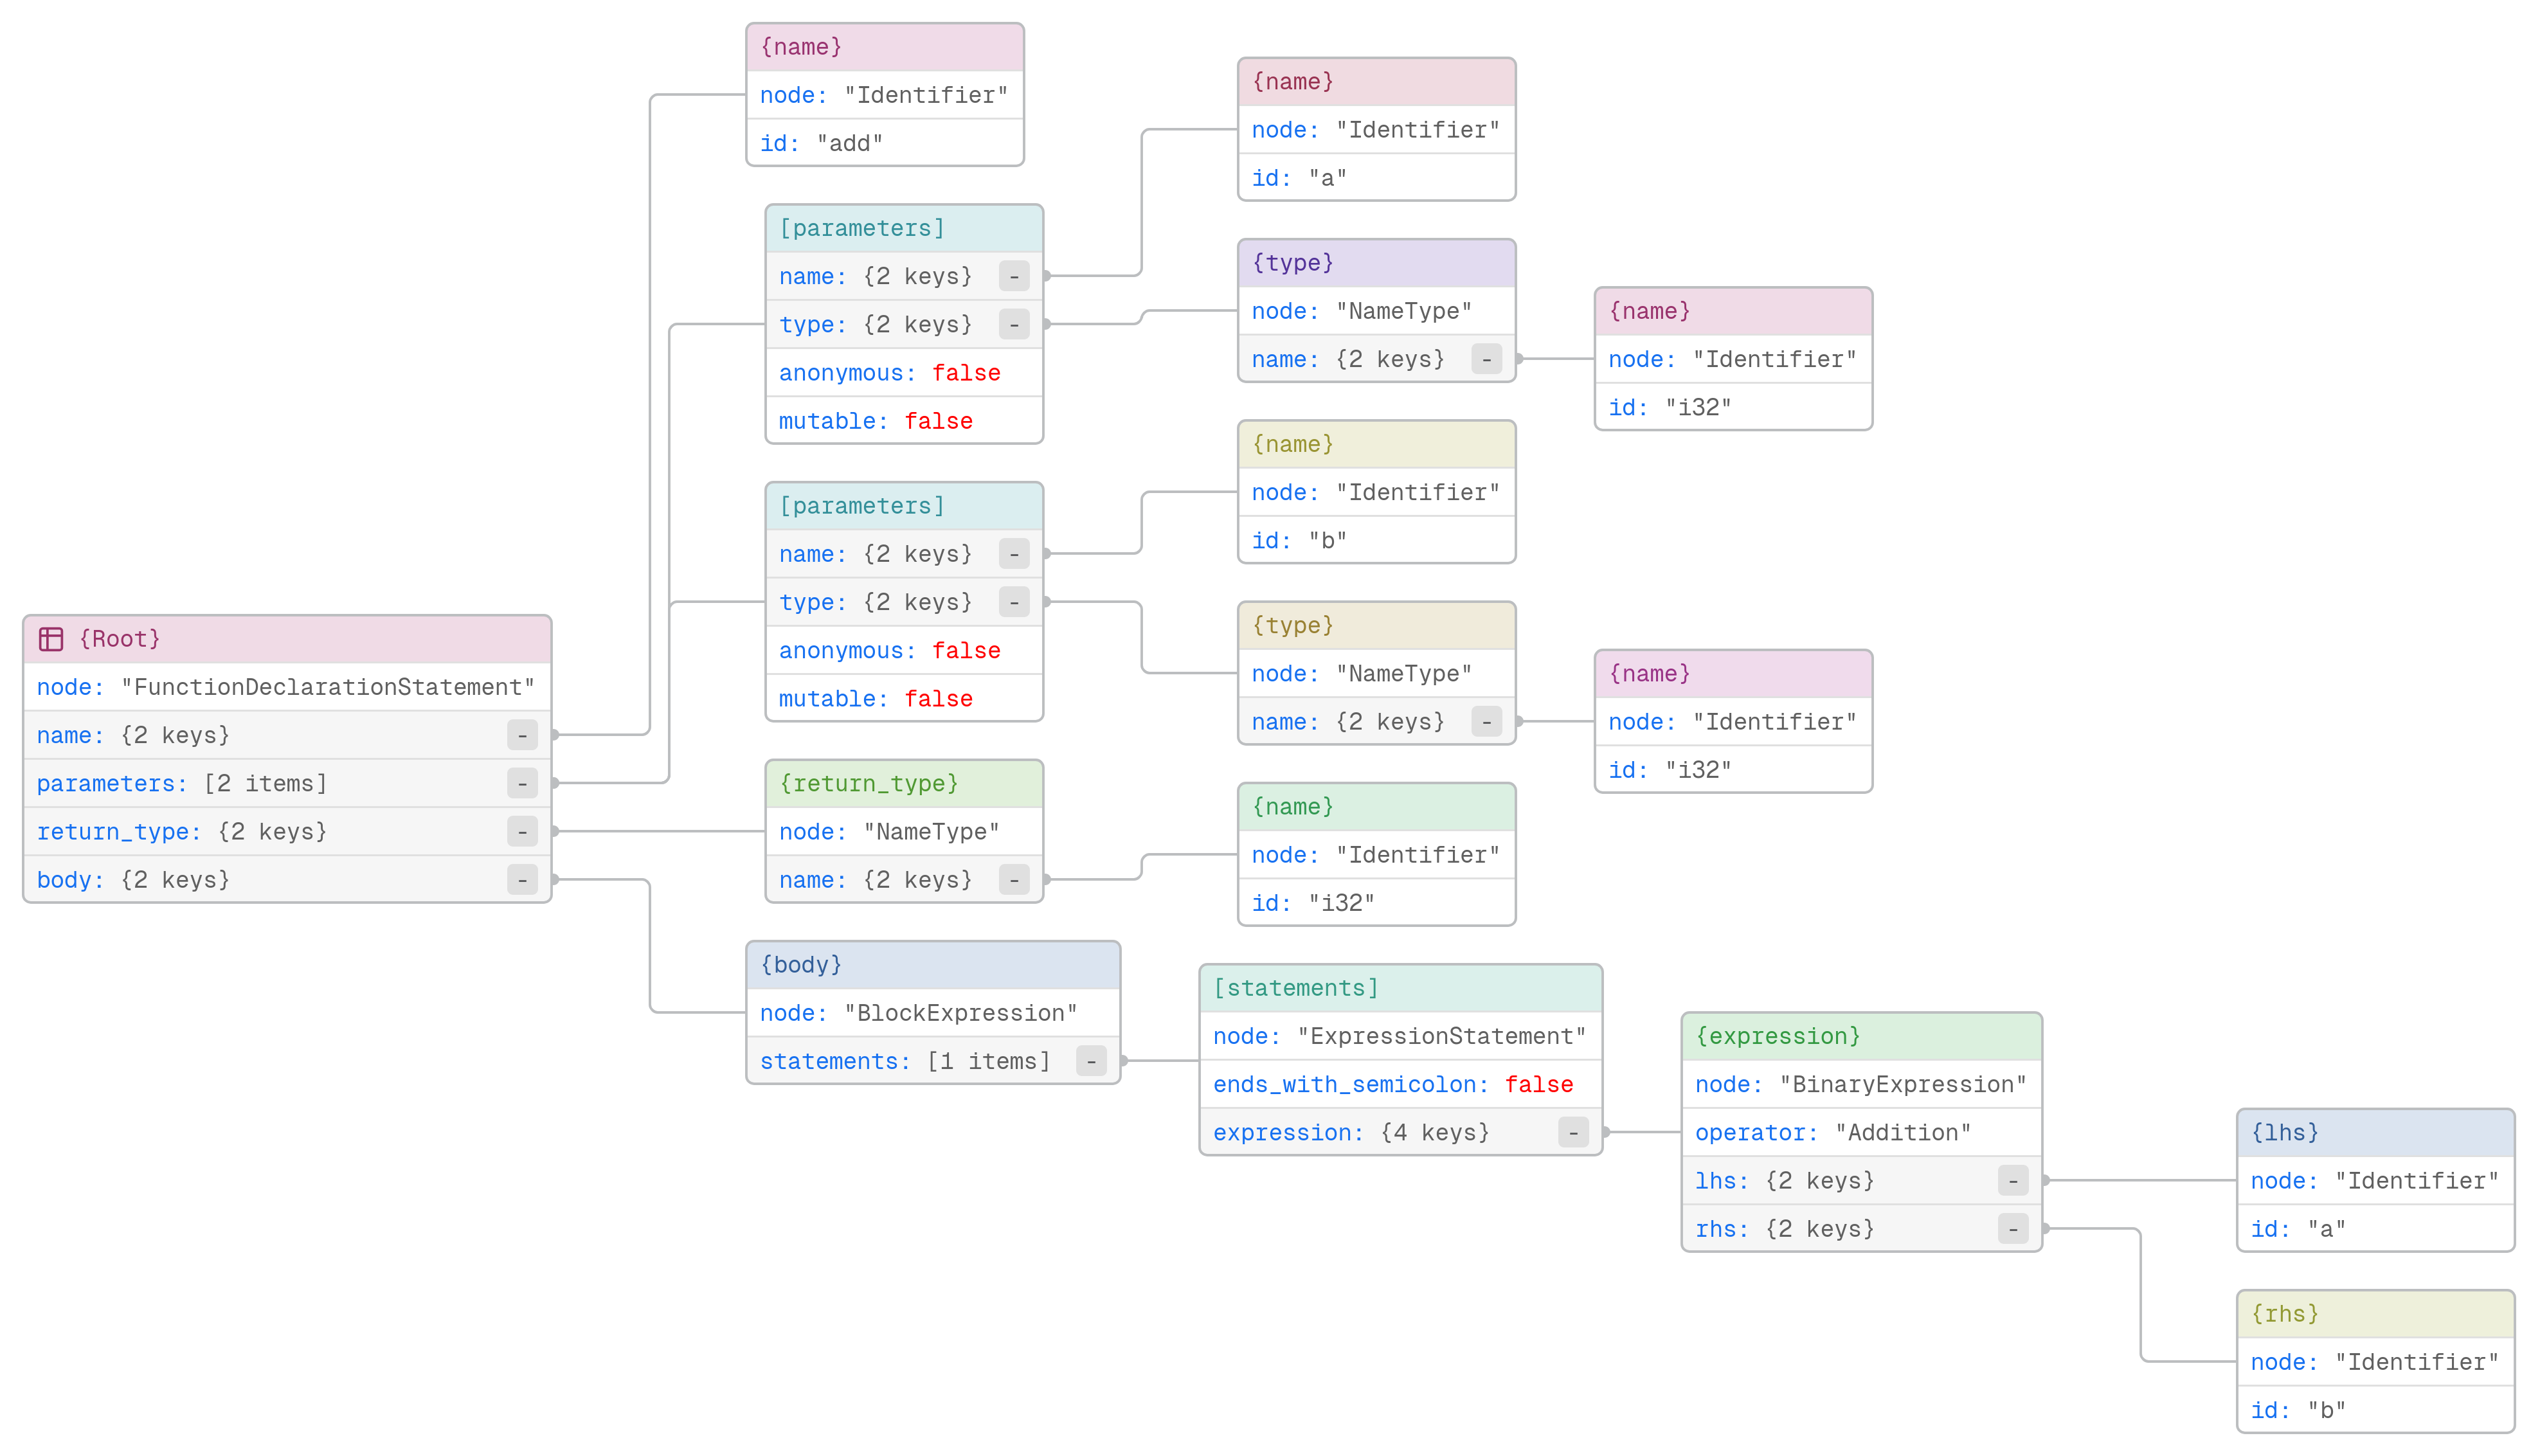
\includegraphics[width=\textwidth]{figures/function_declaration_ast.png}
	\label{fig:bugginout-example-function-declaration-ast}
	\caption{AST generato per la funzione nell'esempio precedente}
\end{figure}
Come possiamo vedere, la radice \`e il nodo \texttt{FunctionDeclarationStatement} che ha come figli:
\begin{itemize}
	\item \texttt{name} (un \texttt{Identifier}): nome della funzione;
	\item \texttt{function\_parameters}: i parametri della funzione, i cui figli sono due nodi, uno per ogni parametro, con a loro volta come figli:
	\begin{itemize}
		\item \texttt{name} (un \texttt{Identifier}): nome del parametro;
		\item \texttt{type} (un \texttt{Type}): tipo del parametro;
		\item \texttt{mutable}: se il parametro \`e mutabile o meno;
		\item \texttt{anonymous}: se il parametro \`e anonimo o meno.
	\end{itemize}
	\item \texttt{return\_type} (un \texttt{Type}): il tipo di ritorno della funzione;
	\item \texttt{body} (una \texttt{BlockExpression}): il corpo della funzione che ha come foglia il nodo \texttt{BinaryExpression} che rappresenta l'espressione \texttt{a + b} e ha come figli:
	\begin{itemize}
		\item \texttt{operator}: che rappresenta l'operatore dell'espressione (in questo caso una somma);
		\item \texttt{lhs} (una \texttt{Expression}, in questo caso specifico un \texttt{Identifier}): la parte sinistra dell'operazione;
		\item \texttt{rhs} (una \texttt{Expression}, in questo caso specifico un \texttt{Identifier}): la parte destra dell'operazione.
	\end{itemize}
\end{itemize}

Un altro esempio interessante \`e la definizione delle espressioni binarie:
\begin{figure}[H]
	\centering
	\begin{minted}[breaklines,frame=lines,fontsize=\footnotesize]{text}
<BinaryExpression> ::=
  <Expression>
  ("+" | "-" | "*" | "/" | "%" | "<<" | ">>" | "<" | ">" | "<=" | ">=" | "==" | "!=" | "&" | "^" | "|" | "&&" | "||")
  <Expression>
	\end{minted}
	\label{fig:bugginout-binary-expression}
	\caption{Grammatica per le espressioni binarie}
\end{figure}

Il motivo per cui ci interessa analizzare questa regola \`e la sua \emph{ambiguit\`a}, ci\`o significa che esistono pi\`u modi d'interpretare la stessa espressione. Ad esempio, l'espressione \texttt{a + b * c} pu\`o essere interpretata in due modi diversi:
\begin{itemize}
	\item \texttt{(a + b) * c}, in cui l'operazione di somma viene eseguita prima della moltiplicazione;
	\item \texttt{a + (b * c)}, in cui l'operazione di moltiplicazione viene eseguita prima della somma.
\end{itemize}
Citando \cite{alfred2007compilers}:
\begin{parcolumns}[colwidths={1=0.44\textwidth,2=0.44\textwidth},rulebetween=true,nofirstindent=true,sloppy=true]{2}
	% LTeX: language=en_us
	\colchunk{
		\leftskip=1em
		``There are two reasons why we might prefer to use the ambiguous grammar. [\ldots] We can easily change the \emph{associativity} and \emph{precedence} of the operators without disturbing the productions or the number of states in the resulting parser.~[\ldots]''
	}
	% LTeX: language=it
	\colchunk{
		\leftskip=1em
		``Ci sono due ragioni per le quali potremmo preferire utilizzare la grammatica ambigua. [\ldots] Possiamo facilmente cambiare l'\emph{associatività} e \emph{precedenza} degli operatori senza disturbare le produzioni o il numero di stati dell'analizzatore grammaticale.~[\ldots]''
	}
	\colplacechunks
\end{parcolumns}

Chiarito il concetto di grammatica e avendone visto alcuni esempi, \`e possibile passare alla discussione dell'analizzatore grammaticale.

In generale un analizzatore grammaticale pu\`o seguire due principali strategie:
\begin{itemize}
	\item \emph{top-down}, in cui l'analizzatore grammaticale inizia dalla radice dell'albero e scende verso le foglie;
	\item \emph{bottom-up}, in cui l'analizzatore grammaticale inizia dalle foglie dell'albero e risale verso la radice.
\end{itemize}
La strategia scelta per BugginOut \`e quella \emph{top-down} per la sua semplicit\`a e facilit\`a d'uso. Pi\`u specificamente, l'analizzatore lessicale \`e un \textit{predictive parser} senza \textit{backtracking} costruito su una grammatica LL(1) \cite{alfred2007compilers}.

Questo significa che, a ogni passo, si sceglie la produzione grammaticale corretta utilizzando solo il prossimo token restituito dall'analizzatore lessicale. \`E importante notare che, per costruire un analizzatore grammaticale di questo tipo, \`e necessario che la grammatica sia priva di \emph{ambiguit\`a} e \emph{ricorsioni sinistre}. La prima condizione \`e stata soddisfatta definendo l'associativit\`a e la precedenza degli operatori\footnote{Lo si vede nel dettaglio nel capitolo \ref{chap:architettura-del-compilatore}.} e la seconda scrivendo meticolosamente la grammatica per evitarle.

Durante l'analisi grammaticale, si potrebbe incorrere in un errore sintattico se un token incontrato durante l'analisi lessicale del programma sorgente non corrisponde a quello che ci si aspetta nella produzione.
\begin{figure}[H]
	\centering
	\begin{minted}[breaklines,linenos,frame=lines,fontsize=\footnotesize]{text}
fn add(a: i32, b: i32): i32 {
  (a + b
}
	\end{minted}
	\begin{minted}[breaklines,frame=lines,fontsize=\footnotesize]{text}
error.bo: Expected "RightParenthesis", got "RightCurlyBracket"!
   3 | }
       ^
	\end{minted}
	\label{fig:bugginout-syntax-error}
	\caption{Errore sintattico generato nel caso di parentesi non bilanciate}
\end{figure}
In questo caso l'analizzatore grammaticale genera un errore e termina l'esecuzione. Questo approccio di gestione degli errori \`e il pi\`u semplice e non \`e in grado di recuperare gli errori\footnote{Su questo tema si spenderanno alcune parole nella sezione \ref{sec:limiti}.}.

\section{Analisi semantica}
\label{sec:analisi-semantica}

L'analisi semantica \`e la fase di compilazione in cui viene verificata la correttezza semantica del programma. In questa fase, l'analizzatore semantico controlla che le operazioni siano valide in base al tipo di dati e alle regole del linguaggio.

I controlli semantici includono:
\begin{itemize}
	\item ordine delle dichiarazioni: verifica che le variabili siano dichiarate prima di essere utilizzate;
	\item ambito (\emph{scope}): verifica che le variabili siano utilizzate all'interno del loro ambito di visibilit\`a;
	\item assegnabilit\`a: verifica se un'espressione \`e assegnabile ad un'altra;
	\item firma delle funzioni: verifica che le funzioni siano chiamate con il numero e il tipo corretto di argomenti;
	\item ...
\end{itemize}
Di tutti i controlli quello che merita una particolare attenzione \`e il \emph{type checking} (controllo dei tipi). Questo controllo verifica che i valori siano usati in maniera coerenti con i loro tipi, ad esempio che non si tenti di assegnare un numero a una stringa o che si assegni un valore booleano a una variabile intera.

Citando \cite{alfred2007compilers}:
\begin{parcolumns}[colwidths={1=0.44\textwidth,2=0.44\textwidth},rulebetween=true,nofirstindent=true,sloppy=true]{2}
	% LTeX: language=en_us
	\colchunk{
		\leftskip=1em
		``To do \emph{type checking} a compiler needs to assign a type expression to each component of the source program. The compiler must then determine that these type expressions conform to a collection of logical rules that is called the \emph{type system} for the source language.

		[\ldots]

		Type checking can take on two forms: synthesis and inference. \emph{Type synthesis} builds up the type of an expression from the types of its sub expressions.~[\dots] \emph{Type inference} determines the type of a language construct from the way it is used.''
	}
	% LTeX: language=it
	\colchunk{
		\leftskip=1em
		``Per fare il \emph{type checking} un compilatore deve assegnare un'espressione di tipo a ciascun componente del programma sorgente. Il compilatore deve quindi determinare che queste espressioni di tipo siano conformi a una collezione di regole logiche che viene chiamata \emph{type sistem} per il linguaggio sorgente.

		[\ldots]

		Il type checking pu\`o assumere due forme: sintesi e inferenza. La \emph{sintesi} costruisce il tipo di un'espressione dai tipi delle sue sottoespressioni.~[\dots] L'\emph{inferenza} determina il tipo di un costrutto del linguaggio dal modo in cui viene utilizzato.''
	}
	\colplacechunks
\end{parcolumns}

Analizziamo ora alcuni esempi di \emph{type checking}.

Di seguito le operazioni per l'analisi semantica di una dichiarazione di variabile:
\begin{enumerate}
	\item si verifica se la dichiarazione specifica un tipo per la variabile in maniera esplicita:
	\begin{itemize}
		\item in tal caso, si passa ad analizzare semanticamente l'espressione che inizializza la variabile e a verificare che abbia lo stesso tipo della variabile (esempio di sintesi del tipo della variabile);
		\item altrimenti, la variabile assume il valore del tipo dell'espressione che la inizializza (esempio d'inferenza del tipo della variabile).
	\end{itemize}
	\item si verifica se la variabile \`e gi\`a stata dichiarata in precedenza usando la \emph{tabella dei simboli}\footnote{Si veda il capitolo \ref{chap:architettura-del-compilatore} per un approfondimento su questo argomento.}.
\end{enumerate}

Di seguito le operazioni per l'analisi semantica di un'espressione \texttt{if}:
\begin{enumerate}
	\item si esegue l'analisi semantica della condizione e si verifica che il tipo dell'espressione sia booleana;
	\item si esegue l'analisi semantica del blocco \texttt{then};
	\item se esiste, si esegue l'analisi semantica del blocco \texttt{else} e si controlla che abbia lo stesso tipo del blocco \texttt{then}.
\end{enumerate}

Di seguito le operazioni per l'analisi semantica di un'espression \texttt{return}:
\begin{enumerate}
	\item si verifica se si restituisce un'espressione:
	\begin{itemize}
		\item in tal caso, si esegue l'analisi semantica dell'espressione e si verifica che il suo tipo sia compatibile con il tipo di ritorno della funzione che si sta analizzando;
		\item altrimenti, si verifica che la funzione abbia tipo di ritorno \texttt{void}.
	\end{itemize}
\end{enumerate}

Durante le operazioni descritte si possono generare errori semantici. Ad esempio, se si tenta di dichiarare una variabile con lo stesso nome di una gi\`a esistente, si genera un errore semantico.

Osserviamone ora qualche esempio:
\begin{figure}[H]
	\centering
	\begin{minted}[breaklines,linenos,frame=lines,fontsize=\footnotesize]{text}
fn add(a: i32): i32 {
  var c = a + b;
  return c;
}
	\end{minted}
	\begin{minted}[breaklines,frame=lines,fontsize=\footnotesize]{text}
not_declared.bo: Unknown identifier
   2 |   var c = a + b;
                     ^
	\end{minted}
	\label{fig:unknown-identifier-error}
	\caption{Errore semantico generato per una variabile non dichiarata}
\end{figure}

\begin{figure}[H]
	\centering
	\begin{minted}[breaklines,linenos,frame=lines,fontsize=\footnotesize]{text}
fn foo(): i32 {
	return 1 + "2";
}
	\end{minted}
	\begin{minted}[breaklines,frame=lines,fontsize=\footnotesize]{text}
invalid_operation.bo: Incompatible types for binary operation
   2 |   return 1 + "2";
                ^^^^^^^
	\end{minted}
	\label{fig:invalid-binary-operation-error}
	\caption{Errore semantico generato per un'operazione non valida}
\end{figure}

\begin{figure}[H]
	\centering
	\begin{minted}[breaklines,linenos,frame=lines,fontsize=\footnotesize]{text}
fn foo(): i32 {
	return "10";
}
	\end{minted}
	\begin{minted}[breaklines,frame=lines,fontsize=\footnotesize]{text}
invalid_return.bo: Incompatible return types
   2 |     return "10";
           ^^^^^^^^^^^^
	\end{minted}
	\label{fig:invalid-return-type-error}
	\caption{Errore semantico generato per un tipo di ritorno non valido}
\end{figure}

\`E importante notare che gli errori semantici sono corretti dal punto di vista della grammatica del linguaggio, ma violano la logica del linguaggio. Trovare questi errori in fase di compilazione, prima dell'esecuzione di un programma, rende il codice pi\`u robusto e riduce il rischio di comportamenti imprevisti.

\section{Generazione del codice}
\label{sec:generazione-del-codice}

La generazione del codice \`e la fase finale della compilazione in cui si traduce il \texttt{CheckedAST} (output dell'analisi semantica) in codice C++ pronto per essere compilato. Il codice generato in C++ ha l'obiettivo di essere leggibile e quanto pi\`u vicino possibile a quello originale, in modo da facilitarne il debug.

Il codice C++ generato \`e composto da:
\begin{itemize}
	\item \emph{prelude}: una serie di dichiarazioni e inclusioni necessarie per il corretto funzionamento del codice generato\footnote{Lo si approfondir\`a nel capitolo \ref{chap:architettura-del-compilatore}.};
	\item prototipi delle funzioni: per ogni funzione dichiarata nel programma BugginOut originale, ne si inserisce il prototipo;
	\item dichiarazioni di funzioni: dopo averne dichiarato i prototipi, si passa a inserirne le implementazioni;
	\item \emph{main}: la funzione principale del programma, costituita da una sola chiamata alla funzione \emph{bo\_main}\footnote{La funzione \texttt{main} deve essere presente in ogni programma BugginOut e in fase di generazione del codice viene rinominata in \texttt{bo\_main} per evitare conflitti con la funzione \texttt{main} prevista dal compilatore C++}.
\end{itemize}

Sebbene una quantit\`a elevata dei nodi generati trova una corrispondenza diretta con il codice C++ generato, alcuni nodi meritano un particolare approfondimento: i tipi, l'espressioni \texttt{if} e i blocchi.

Per la traduzione dei tipi, si effettuano le seguenti operazioni:
\begin{itemize}
	\item i tipi primitivi vengono tradotti cos\`i come sono grazie a degli alias definiti dal \emph{prelude};
	\item gli \emph{array} vengono tradotti in \texttt{std::array};
	\item gli \emph{slice} vengono tradotti in \texttt{std::span};
	\item i range vengono tradotti nel tipo \texttt{bo\_range} definito nel \emph{prelude}\footnote{Si veda il capitolo \ref{chap:architettura-del-compilatore} per un approfondimento su questo tipo.};
	\item i puntatori vengono tradotti usando la sintassi dei puntatori C++ (ovvero \texttt{type*})\footnote{\`E bene notare che quindi un puntatore, \emph{weak} o \emph{strong} che sia, viene tradotto nello stesso tipo. \`E possibile farlo in quanto la compatibilit\`a dei tipi \`e garantita dalla fase di analisi semantica.};
\end{itemize}

Le espressioni \texttt{if}, invece, meritano un trattamento speciale nel caso in cui queste siano usate come espressione, ad esempio se si deve tradurre:
\begin{figure}[H]
	\centering
	\begin{minted}[breaklines,frame=lines,fontsize=\footnotesize]{text}
var x = if (a > b) { a } else { b };
	\end{minted}
	\label{fig:bugginout-if-expression}
	\caption{Esempio di espressione \texttt{if} in BugginOut usata come espressione}
\end{figure}
Per tradurre questo tipo di espressione, non supportata nativamente dal C++, si fa uso dell'estensione \emph{compound statements} del compilatore GNU\footnote{Di questo si parler\`a meglio nel capitolo \ref{chap:conclusioni}.} per tradurre l'espressione in un blocco di codice che restituisce il valore corretto:
\begin{figure}[H]
	\centering
	\begin{minted}[breaklines,frame=lines,fontsize=\footnotesize]{cpp}
i32 const x = (({
    i32 __block_ret_1 {};
    if (static_cast<bool>((a)>(b)))
    {
        __block_ret_1 = a;
    }
    else
    {
        __block_ret_1 = ({
            b;
        });
    }
    __block_ret_1;
}));
	\end{minted}
	\label{fig:bugginout-if-expression-transpiled}
	\caption{Traduzione dell'esempio precedente in C++}
\end{figure}
In questo modo, l'espressione \texttt{if} viene tradotta in un blocco di codice che memorizza il valore corretto in una variabile restituita alla fine di esso.

Un discorso analogo vale per i blocchi di codice, per fare un esempio, il seguente blocco di codice
\begin{figure}[H]
	\centering
	\begin{minted}[breaklines,frame=lines,fontsize=\footnotesize]{text}
var y = {
    var x = 1;
    x + 2
}
	\end{minted}
	\label{fig:bugginout-block-expression}
	\caption{Esempio di blocco che restituisce un valore in BugginOut}
\end{figure}
viene tradotto in C++ come:
\begin{figure}[H]
	\centering
	\begin{minted}[breaklines,frame=lines,fontsize=\footnotesize]{cpp}
i32 const y = ({
    i32 const x = (static_cast<i32>(1));
    static_cast<i32>((x)+(static_cast<i32>(2)));
});
	\end{minted}
	\label{fig:bugginout-block-expression-transpiled}
	\caption{Traduzione dell'esempio precedente in C++}
\end{figure}

Una volta generato il codice C++, questo viene memorizzato in un file con estensione \texttt{.cpp} e, successivamente, compilato usando il compilatore GNU C++ per produrre un eseguibile\footnote{Si veda il capitolo \ref{chap:architettura-del-compilatore} per un approfondimento su questo argomento.}.

	% LTeX: language=it

\chapter{Architettura del compilatore}
\label{chap:architettura-del-compilatore}

\begin{figure}[H]
	\centering
	\scalebox{0.8}{\begin{tikzpicture}[node distance=2cm]
		\node (source) [draw, rectangle, text centered, minimum width=4cm, minimum height=1cm, rounded corners] {Codice sorgente};
		\node (lexer) [below of=source, draw, rectangle, text centered, minimum width=3cm, minimum height=1cm] {\texttt{Lexer}};
		\node (parser) [below of=lexer, draw, rectangle, text centered, minimum width=3cm, minimum height=1cm] {\texttt{Parser}};
		\node (typechecker) [below of=parser, draw, rectangle, text centered, minimum width=3cm, minimum height=1cm] {\texttt{Typechecker}};
		\node (transpiler) [below of=typechecker, draw, rectangle, text centered, minimum width=3cm, minimum height=1cm] {\texttt{Transpiler}};
		\node (output) [below of=transpiler, draw, rectangle, text centered, minimum width=4cm, minimum height=1cm, rounded corners] {Codice C++ generato};

		\draw [->] (source) -- (lexer);
		\draw [->] (lexer) to node[left] {\texttt{Token}s} (parser);
		\draw [->] (parser) to node[left] {\texttt{AST}} (typechecker);
		\draw [->] (typechecker) to node[left] {\texttt{CheckedAST}} (transpiler);
		\draw [->] (transpiler) -- (output);
	\end{tikzpicture}}
	\caption{Moduli del processo di compilazione}
	\label{fig:moduli-compilatore}
\end{figure}

Nel seguente capitolo si descrive l'architettura del compilatore BugginOut, affrontando i moduli che lo compongono e le fasi del compilatore che realizzano. Nella figura sopra si pu\`o osservare l'architettura ad alto livello del compilatore che \`e costituito da quattro moduli principali:
\begin{itemize}
	\item \texttt{Lexer}: realizza l'analisi lessicale;
	\item \texttt{Parser}: realizza l'analisi sintattica;
	\item \texttt{Typechecker}: realizza l'analisi semantica;
	\item \texttt{Transpiler}: realizza la generazione del codice C++.
\end{itemize}
Questi interagiscono secondo un modello a \textit{pipeline}, in cui l'output di un modulo \`e l'input del successivo. Nel seguito si descriver\`a ciascuno di questi moduli e ci\`o che producono.

\section{\texttt{Lexer}}
\label{sec:lexer}

\begin{figure}[H]
	\centering
	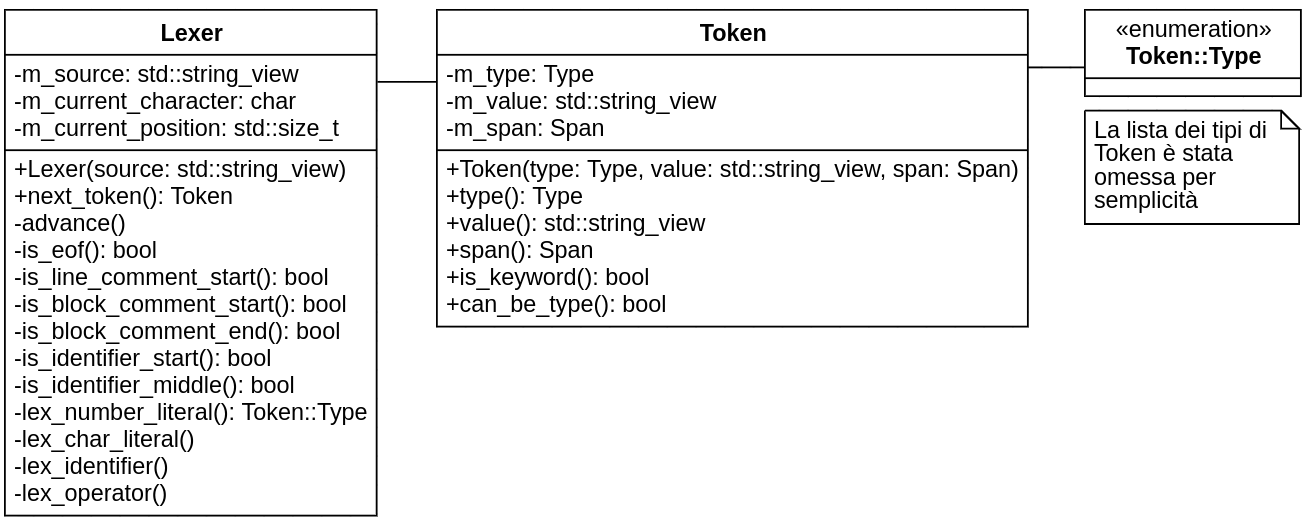
\includegraphics[width=0.9\textwidth]{figures/lexer.png}
	\caption{Diagramma UML del \texttt{Lexer}}
	\label{fig:lexer-uml}
\end{figure}

L'analisi lessicale \`e realizzata per mezzo di due classi: \texttt{Token} e \texttt{Lexer}.

La classe \texttt{Token} rappresenta i token generati dall'analisi lessicale ed \`e costituito da:
\begin{itemize}
	\item \texttt{type}: il tipo del token (un valore dell'enumerazione \texttt{Token::Type});
	\item \texttt{value}: il valore del token (una stringa);
	\item \texttt{span}: la posizione del token nel codice sorgente (un oggetto di tipo \texttt{Span}\footnote{Questo tipo di oggetto rappresenta una posizione all'interno del codice sorgente ed \`e non altro che un intervallo di due indici nella stringa contenente il sorgente del programma.}).
\end{itemize}

La classe \texttt{Lexer} realizza l'automa a stati finiti discusso nella sezione \ref{sec:analisi-lessicale} memorizzando:
\begin{itemize}
	\item \texttt{source}: il codice sorgente da analizzare (una stringa);
	\item \texttt{current\_character}: il carattere da analizzare (un carattere);
	\item \texttt{current\_position}: la posizione del prossimo carattere da analizzare (un intero).
\end{itemize}
Il metodo \texttt{advance} permette di avanzare l'automa al prossimo carattere, aggiornando \texttt{current\_character} e \texttt{current\_position} e, inoltre, di controllare se si \`e raggiunti la fine del codice sorgente. In tal caso, il metodo imposta \texttt{current\_character} al valore speciale $-1$.

Con il metodo \texttt{next\_token} \`e possibile avanzare l'automa e generare il prossimo token. Ogni volta che questo metodo viene chiamato si occuper\`a di:
\begin{itemize}
	\item rimuovere spazi vuoti e commenti;
	\item analizzare \texttt{current\_character} e generare il token corrispondente o generare un errore se il carattere non \`e valido.\footnote{Per la gestione degli errori si veda la sezione \ref{sec:gestione-degli-errori}}
\end{itemize}
In base al carattere incontrato, si delega il compito dell'analisi lessicale ad uno dei metodi presenti nel diagramma. Ad esempio, se il carattere incontrato \`e un numero si richiamer\`a il metodo \texttt{lex\_number\_literal}. Questo permette di mantenere il codice del \texttt{Lexer} pulito e facilmente estendibile, poich\'e ogni metodo si occupa di un caso specifico.

\section{\texttt{Parser}}
\label{sec:parser}

\begin{figure}[H]
	\centering
	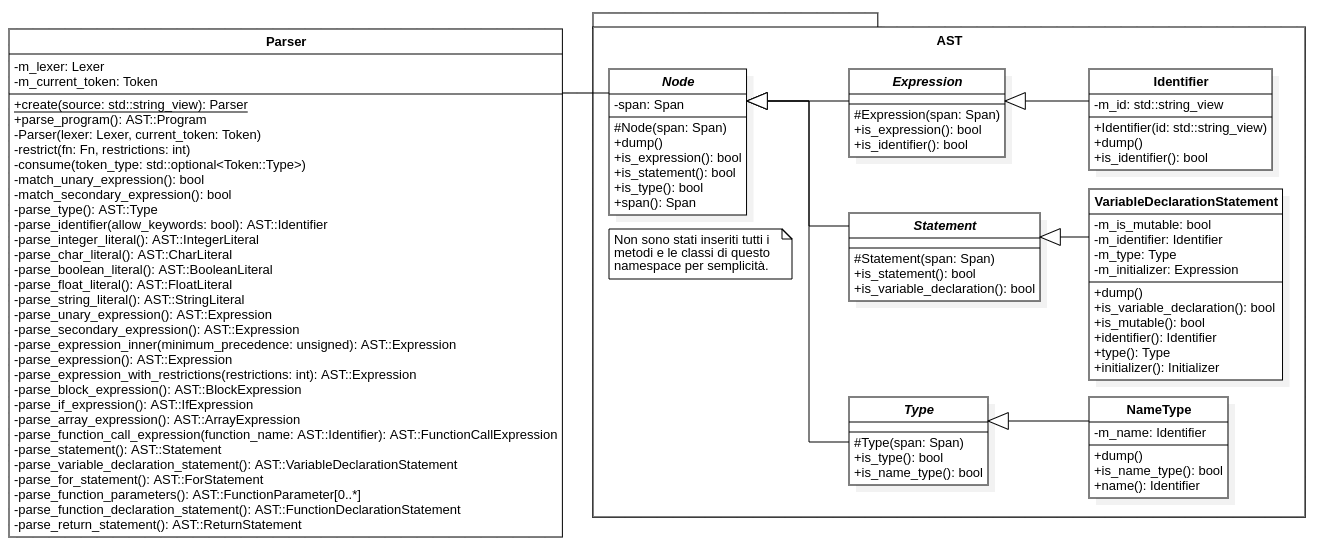
\includegraphics[width=0.9\textwidth]{figures/parser.png}
	\caption{Diagramma UML del \texttt{Parser}}
	\label{fig:parser-uml}
\end{figure}

L'analisi grammaticale \`e gestita dalla classe \texttt{Parser} che genera l'AST, rappresentato nell'omonimo \textit{namespace}, a partire dai token genrati dal \texttt{Lexer}.

Partiamo dal descrivere il \textit{namespace} \texttt{AST}. Questo contiene la classe madre \texttt{Node} che rappresenta un generico nodo dell'AST. L'unico suo attributo \`e \texttt{span}, la posizione nel codice sorgente. Da essa derivano le seguenti classi astratte:
\begin{itemize}
	\item \texttt{Expression}: rappresenta un'espressione, ovvero un nodo che restituisce un valore;
	\item \texttt{Statement}: rappresenta uno italiano, ovvero un nodo che non restituisce un valore;
	\item \texttt{Type}: rappresenta un tipo di dato.
\end{itemize}
Da ciascuna di queste a loro volta, derivano tutte le classi che rappresentano i nodi dell'AST. Ad esempio, come \`e possibile osservare nella figura \ref{fig:parser-uml}, possiamo osservare tre nodi:
\begin{itemize}
	\item \texttt{Identifier}: sottoclasse di \texttt{Expression}, rappresenta un identificatore ed \`e descritto dall'attributo stringa \texttt{id}.
	\item \texttt{VariableDeclarationStatement}: sottoclasse di \texttt{Statement}, rappresenta una dichiarazione di variable ed \`e descritto dagli attributi:
	\begin{itemize}
		\item \texttt{is\_mutable}: un booleano che indica se la variabile \`e mutabile o meno;
		\item \texttt{identifier}: il nome della variabile (un oggetto di tipo \linebreak \texttt{Identifier});
		\item \texttt{type}: il tipo della variabile (un oggetto di tipo \texttt{Type});
		\item \texttt{initializer}: l'inizializzatore della variabile (un oggetto di tipo \texttt{Expression}).
	\end{itemize}
	\item \texttt{NameType}: sottoclasse di \texttt{Type}, rappresenta un tipo di dato descritto da un singolo identificatore, il quale sar\`a un tipo primitivo (ad esempio: \texttt{i32} o \texttt{char}).
\end{itemize}

\`E bene notare che la classe \texttt{Node} definisce una serie di metodi importanti:
\begin{itemize}
	\item il metodo \texttt{dump} che permette di stampare in formato JSON l'intera struttura del nodo; questo risulta utile in fase di debugging per verificare l'AST generato dal \texttt{Parser}.
	\item i metodi \mbox{\texttt{is\_expression}, \texttt{is\_statement} e \texttt{is\_type}} che permettono di verificare il tipo di nodo; questi metodi sono utili per effettuare controlli e conversioni di tipo durante l'analisi semantica e la generazione del codice.
\end{itemize}

Come anticipato nella sezione \ref{sec:analisi-grammaticale}, la grammatica di questo linguaggio \`e LL(1) e, citando \cite{alfred2007compilers}:
\begin{parcolumns}[colwidths={1=0.44\textwidth,2=0.44\textwidth},rulebetween=true,nofirstindent=true,sloppy=true]{2}
	% LTeX: language=en_us
	\colchunk{
		\leftskip=1em
		``The first ``L'' in LL(1) stands for scanning the input from left to right, the second ``L'' for producing a leftmost derivation, and the ``1'' for using one input symbol of \emph{lookahead} at each step to make parsing action decisions.''
	}
	% LTeX: language=it
	\colchunk{
		\leftskip=1em
		``La prima ``L'' in LL(1) indica che si analizza l'input da sinistra verso destra, la seconda ``L'' indica che si produce una derivazione sinistra e l'``1'' per usare un \emph{lookahead} di un simbolo d'input a ogni passo per fare decisioni di analisi grammaticale.''
	}
	\colplacechunks
\end{parcolumns}

I parser costruiti per questo tipo di grammatica, e di conseguenza quella di BugginOut, sono detti \emph{predictive}, ovvero dei parser \emph{recursive descent} senza il bisogno di \emph{backtracking}. I parser \emph{recursive descent} sono dei particolari parser \emph{top-down} costruiti con delle procedure ricorsive dove ognuna di queste riflette un non-terminale della grammatica. Si \`e scelto di costruire il parser seguendo questo approccio proprio perch\'e il codice che ne risulta \`e molto semplice, leggibile ed efficiente, non essendo richiesto il backtracking. Di fatti, gli unici due attributi richiesti per mantenere lo stato del parser sono:
\begin{itemize}
	\item \texttt{lexer}: il \texttt{Lexer} che fornisce i token da analizzare;
	\item \texttt{current\_token}: il token corrente da analizzare.
\end{itemize}

Ogni metodo del parser, che rappresenta un non-terminale della grammatica, analizzer\`a il token corrente e, se corretto, lo \emph{consumer\`a}. Questa operazione viene implementata dal metodo \texttt{consume} e corrisponde ad ottenere il prossimo token dal \texttt{Lexer} e aggiornare \texttt{current\_token}. Il metodo prevede un parametro opzionale che permette di specificare il tipo di token atteso. Se il token corrente non corrisponde al tipo atteso, viene generato un errore di sintassi. Se il tipo di token non viene specificato, il metodo consuma il token corrente.

\`E importante notare che per realizzare dei \emph{predictive parser} la grammatica deve soddisfare due requisiti molto importanti:
\begin{itemize}
	\item non deve contenere ricorsioni sinistre;
	\item non deve essere ambigua.
\end{itemize}

La grammatica, per come \`e stata definita, non contiene ricorsioni sinistre ma \`e ambigua nella gestione delle espressioni e dei loro operatori. Questo \`e stato fatto volutamente per due ragioni:
\begin{itemize}
	\item \`e possibile cambiare la precedenza ed associativit\`a degli operatori in modo semplice, senza dover modificare la grammatica;
	\item il parser non spende tempo utile nell'analizzare produzioni \textit{singole} ovvero costituite da un solo non-terminale.
\end{itemize}
In ogni caso, l'amgiguit\`a deve essere gestita e, per farlo, si utilizza un algoritmo di \emph{precedence climbing}.

Introdotto per la prima volta da \cite{barron1981bcpl}, l'idea alla base \`e quella di avere una funzione ricevere in input un'espressione e una \emph{precedenza minima}. Durante l'analisi, la funzione consuma gli operandi fino a quando incontra operatori la cui precedenza \`e maggiore o uguale a quella minima. Se un operatore ha precedenza inferiore, l'espressione si interrompe e si ritorna al livello di ricorsione precedente. L'associativit\`a di un operatore viene gestita in maniera molto elegante, con un semplice controllo effettuato prima della prossima chiamata ricorsiva: se l'operatore \`e associativo a sinistra allora ne aumenta di un'unit\`a la precedenza, altrimenti la lascia invariata. Per capire meglio come funziona, vediamo degli esempi:
\begin{itemize}
	\item Si supponga di voler analizzare l'espressione \texttt{a + b + c}, che la precedenza di \texttt{+} sia 2 e che \texttt{+} sia associativo a sinistra.

	La prima chiamata ricorsiva consuma \texttt{a} e chiama la funzione con precedenza minima $2 + 1$ essendo \texttt{+} associativo a sinistra. La prossima chiamata trover\`a nuovamente \texttt{+} con precedenza $2$ minore della precedenza minima $2 + 1$. Allora esce e l'espressione generata sar\`a \linebreak \texttt{(a + b) + c}.
	\item Adesso si supponga di essere nelle stesse condizioni dell'esempio precedente con l'unica differenza che \texttt{+} sia associativo a destra.

	Durante l'analisi la seconda chiamata alla funzione avr\`a precedenza minima $2$ e, dunque, quando incontrer\`a \texttt{+} lo consumer\`a e l'espressione generata sar\`a \texttt{a + (b + c)}.
\end{itemize}

Questo algoritmo \`e implementato tramite tre funzioni:
\begin{itemize}
	\item \texttt{parse\_expression\_inner}: \`e la funzione ricorsiva di cui si \`e discusso fino ad ora;
	\item \texttt{parse\_primary\_expression}: \`e la funzione che analizza il non-terminale \texttt{<primary>};
	\item \texttt{parse\_secondary\_expression}: \`e la funzione che, prese la parte sinistra e l'operatore di un'espressione ottenuti da \linebreak \texttt{parse\_expression\_inner}, analizza la parte destra (se necessario) e li combina per ottenere l'espressione intermedia.
\end{itemize}
Per gestire la precedenza e l'associativit\`a degli operatori si usa una classe ausiliaria detta \texttt{OperatorData} che mantiene questi due valori per ognuno degli operatori. Per rappresentare la precedenza si usa un intero senza segno che, se basso indica una bassa precedenza, se alto indica una alta precedenza. Per l'associativit\`a si usa una semplice enumerazione di due valori: \texttt{Left} se a sinistra e \texttt{Right} se a destra.

\section{\texttt{Typechecker}}
\label{sec:typechecker}

L'analisi semantica \`e realizzata con la classe \texttt{Typechecker} che si occupa di arrichire l'AST, generando il \texttt{CheckedAST}, con le informazioni di tipo rappresentate nel \textit{namespace} \texttt{Types}.

\begin{figure}[H]
	\centering
	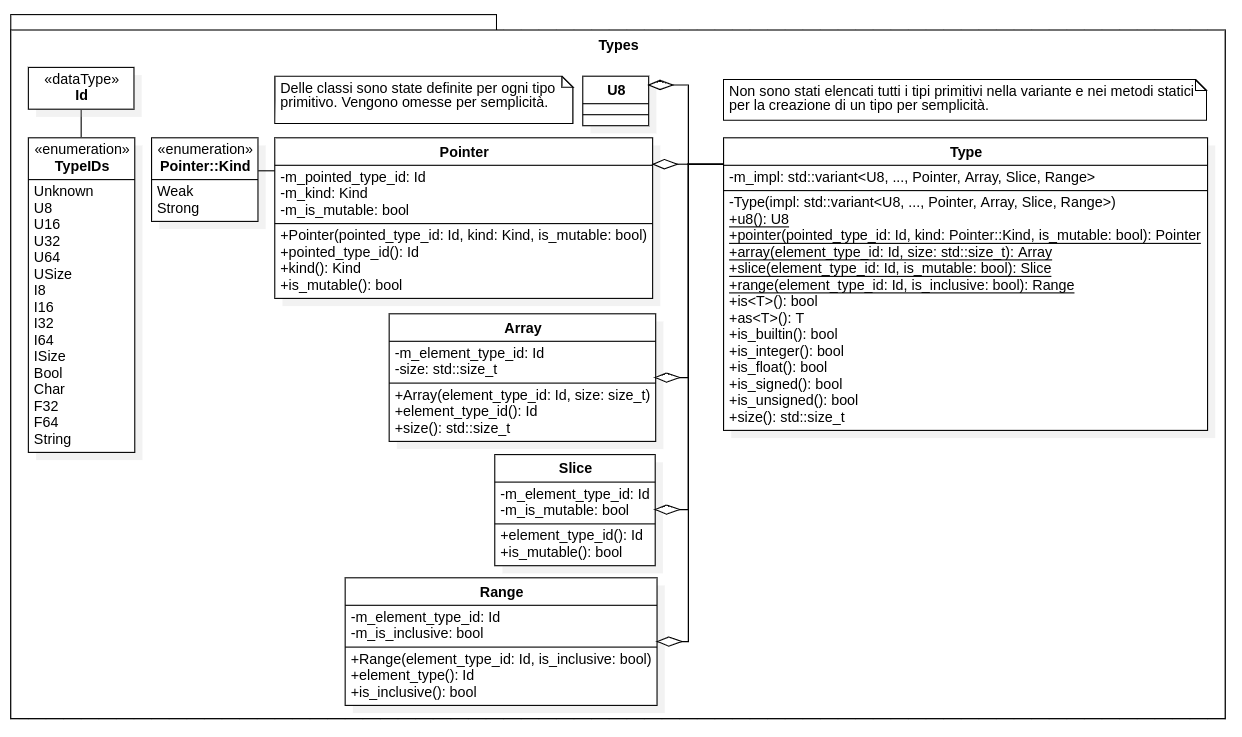
\includegraphics[width=0.9\textwidth]{figures/types.png}
	\caption{Diagramma UML del \textit{namespace} \texttt{Types}}
	\label{fig:typechecker-types}
\end{figure}

Il \textit{namespace} \texttt{Types} si occupa del \emph{type system} e contiene:
\begin{itemize}
	\item delle classi vuote per ogni tipo primitivo (\texttt{U8}, \texttt{U16}, ...);
	\item le classi \texttt{Pointer}, \texttt{Array}, \texttt{Slice} e \texttt{Range} per i rispettivi tipi;
	\item la classe \texttt{Type}.
\end{itemize}
Le classi per i tipi composti contengono ciasuna le propriet\`a relative al tipo rappresentato. Ad esempio, la classe \texttt{Array} memorizza la dimensione e il tipo degli elementi, mentre \texttt{Range} memorizza il tipo dell'intervallo e se l'estremo superiore \`e incluso.

La classe \texttt{Type} funge da \textit{wrapper} attorno ad un \textit{sum-type} che rappresenta un'unione disgiunta di tutte le classi viste sopra. L'adozione di un \textit{sum-type}, anzich\'e di una gerarchia di classi, consente una maggiore \textit{type safety} e una rappresentazione pi\`u efficiente senza allocazioni sull'\textit{heap}.

La clase \texttt{Type} definisce dei metodi per creare dei tipi specifici (ad esempio, \texttt{u8}, \texttt{pointer}, \texttt{array}, ...), nonch\'e dei metodi di introspezione (ad esempio, \texttt{is}, \texttt{is\_integer}, \texttt{size}, ...) utili per verificare la propriet\`a di un tipo. Infine, fornisce il metodo \texttt{as} per accedere direttamente alla rappresentazione concreta del tipo.

\begin{figure}[H]
	\centering
	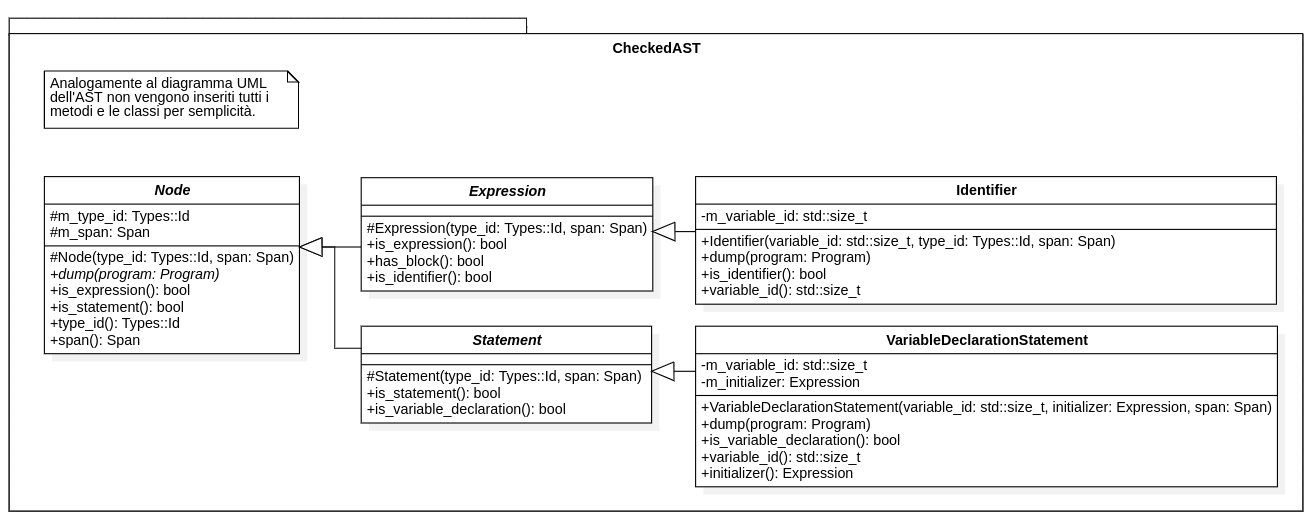
\includegraphics[width=0.9\textwidth]{figures/checked_ast.png}
	\caption{Diagramma UML del \textit{namespace} \texttt{CheckedAST}}
	\label{fig:checked-ast-uml}
\end{figure}

Il \texttt{CheckedAST} \`e una struttura analoga all'\texttt{AST} originale, ma arricchita con informazioni di tipo. L'arricchimento consiste nell'aggiunta, in ciascun \texttt{Node}, di un attributo \texttt{type} di tipo \texttt{Types::Id}. Quest'ultimo rappresenta un identificatore numerico univoco del tipo, il cui significato sarà chiarito nel paragrafo dedicato alla classe \texttt{Typechecker}. Una differenza sostanziale rispetto all'\texttt{AST} è la rimozione del sottoalbero di classi \texttt{Type}, le cui informazioni vengono ora riassunte tramite l'identificatore del tipo.

\begin{figure}[H]
	\centering
	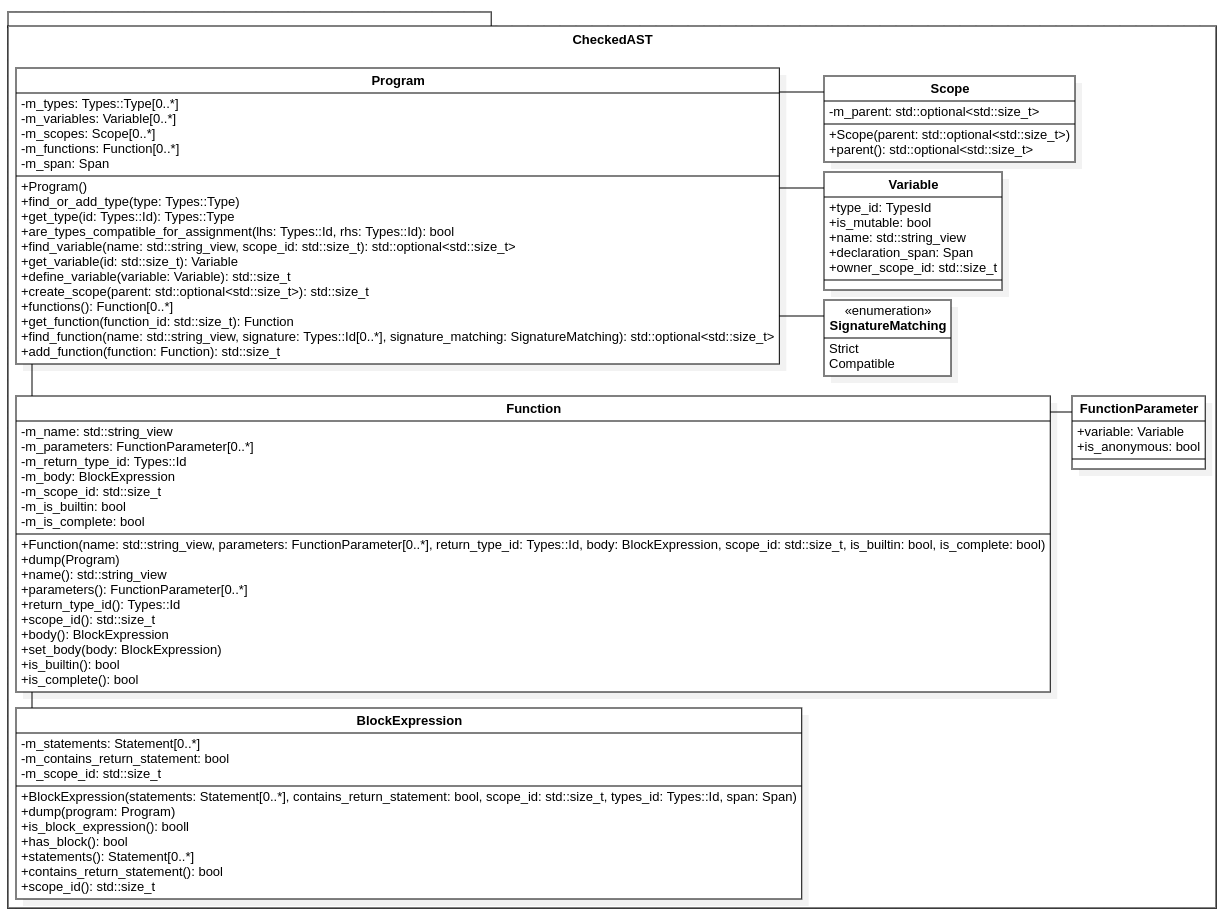
\includegraphics[width=0.9\textwidth]{figures/checked_ast_program.png}
	\caption{Diagramma UML della classe \texttt{CheckedAST::Program}}
	\label{fig:checked-ast-program-uml}
\end{figure}

All'interno del \texttt{CheckedAST} viene definita la classe \texttt{Program}. Questa \`e particolarmente importante in quanto contiene una serie di attributi che cade sotto il termine ombrello di \emph{tabella dei simboli}:
\begin{itemize}
	\item \texttt{scopes}: \`e una lista di oggetti di tipo \texttt{Scope} che rappresentano gli \emph{scope} (ambito di visibilit\`a) del programma, ovvero la porzione di codice in cui una variabile \`e visibile e utilizzabile; ognuno di questi contiene un riferimento opzionale allo \textit{scope} genitore.
	\item \texttt{functions}: \`e una lista di oggetti di tipo \texttt{Function} che contiene tutte le funzioni dichiarate nel programma, costituite da:
	\begin{itemize}
		\item \texttt{name}: il nome della funzione;
		\item \texttt{parameters}: una lista di oggetti di tipo \texttt{FunctionParameter} che rappresentano i parametri della funzione, ognuno dei quali contiene un oggetto di tipo \texttt{Variable} che rappresenta la sua dichiarazione e un booleano che indica se \`e \emph{anonimo};
		\item \texttt{return\_type}: l'identificatore del tipo di ritorno della funzione;
		\item \texttt{body}: il corpo della funzione, un oggetto di tipo \texttt{BlockExpression};
		\item \texttt{scope\_id}: l'identificatore dello \textit{scope} dei parametri della funzione.
		\item \texttt{is\_builtin}: un booleano che indica se \`e una funzione predefinita del linguaggio;
		\item \texttt{is\_complete}: un booleano che indica se la funzione \`e completa o meno; una funzione \`e considerata completa se il suo corpo \`e stato analizzato.
	\end{itemize}
	\item \texttt{variables}: è una lista di oggetti di tipo \texttt{Variable} che contengono informazioni sulle variabili dichiarate nel programma e sono:
	\begin{itemize}
		\item \texttt{type\_id}: l'ID del tipo della variabile;
		\item \texttt{is\_mutable}: un booleano che indica se la variabile \`e mutabile o meno;
		\item \texttt{name}: il nome della variabile;
		\item \texttt{declaration\_span}: la posizione della dichiarazione della variabile;
		\item \texttt{owner\_scope\_id}: l'ID dello \emph{scope} della variabile.
	\end{itemize}
\end{itemize}

\begin{figure}[H]
	\centering
	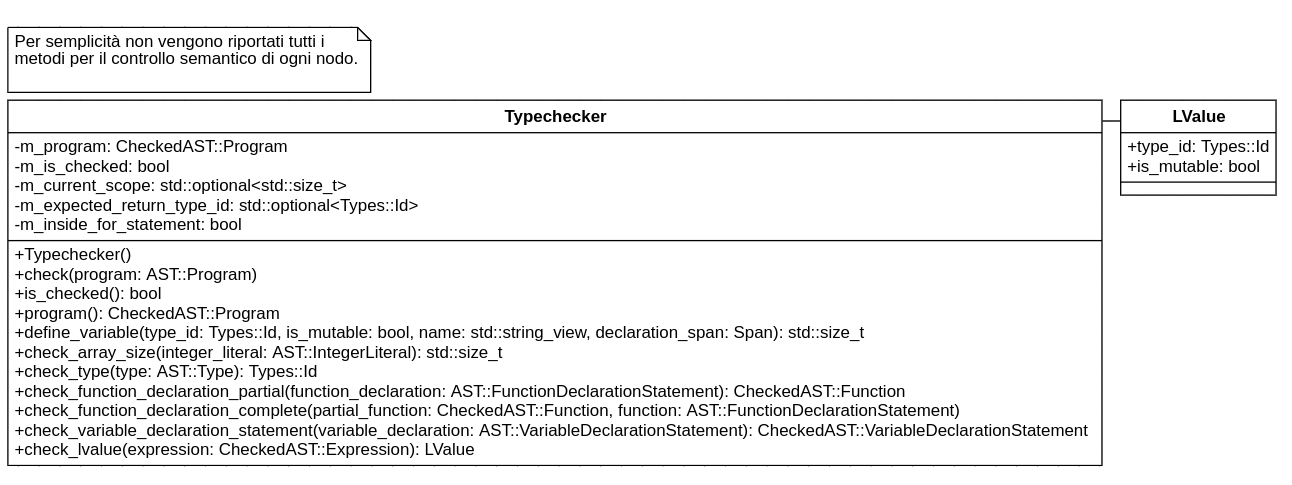
\includegraphics[width=0.9\textwidth]{figures/typechecker.png}
	\caption{Diagramma UML della classe \texttt{Typechecker}}
	\label{fig:typechecker-uml}
\end{figure}

Una volta delineate le basi strutturali del \texttt{Typechecker}, si pu\`o passare a descrivere il suo compito e funzionamento. Oltre che di costruirlo, si occupa di fare i controlli semantici sul programma. L'approccio utilizzato \`e il \emph{bidirectional typechecking}, introdotto da \cite{pierce2000local}.
\begin{parcolumns}[colwidths={1=0.44\textwidth,2=0.44\textwidth},rulebetween=true,nofirstindent=true,sloppy=true]{2}
	% LTeX: language=en_us
	\colchunk{
		\leftskip=1em
		``[\dots] the typechecker operates two distinct modes: \emph{synthesis} mode, where typing information is propagated upward from subexpressions, and \emph{checking} mode, where information is propagated downward from enclosing expressions. Synthesis mode [\dots] is used when we do not know anything about the expected type of an expression [\dots]. Checking mode is used when the surrounding context determines the type of the expression and we only need to check that it does have that type.''
	}
	% LTeX: language=it
	\colchunk{
		\leftskip=1em
		``[\dots] il typechecker opera in due modalit\`a distinte: la modalit\`a di \emph{sintesi}, dove le informazioni di tipo vengono propagate verso l'alto dalle sottoespressioni, e la modalit\`a di \emph{controllo}, dove le informazioni vengono propagate verso il basso dalle espressioni pi\`u esterne. La modalit\`a di sintesi [\dots] \`e usata quando non sappiamo nulla sul tipo atteso di un'espressione [\dots]. La modalit\`a di controllo \`e usata quando il contesto circostante determina il tipo dell'espressione e bisogna solo controllare che abbia quel tipo.''
	}
	\colplacechunks
\end{parcolumns}

In seguito ci riferiremo alla modalit\`a di controllo con \emph{check} e a quella di sintesi con \emph{infer}, per riflettere meglio la terminologia usata nel \texttt{Typechecker}.

Ogni nodo del \texttt{CheckedAST} viene verificato tramite un metodo \texttt{check} apposito che si occupa di verificarne la correttezza semantica, richiamando ricorsivamente i metodi \texttt{check} per ogni nodo figlio fino a quando non si raggiungono le foglie. Eseguiti tutti i controlli semantici, se questi hanno avuto successo, il metodo restituisce il nodo corrispondente del \texttt{CheckedAST}, altrimenti si genera un errore semantico.

Attualmente, il \texttt{Typechecker} effettua una sola operazione di tipo \textit{infer}. Questa si trova nella gestione delle dichiarazioni delle variabili con tipo implicito. In questo caso, si analizzer\`a l'inizializzatore della variabile con una chiamata a \texttt{check\_expression} e, in caso di successo, si otterr\`a il tipo dell'espressione. Questo tipo viene dunque utilizzato come tipo della variabile dichiarata.\footnote{Sull'inferenza, e come questa pu\`o essere utilizata nel futuro del linguaggio, si discuter\`a nelle conclusioni.}

\begin{figure}[H]
	\centering
	\begin{minted}[breaklines,frame=lines,fontsize=\footnotesize]{text}
fn foo(): i32 { 42 }

fn main(): void {
    var a = foo();
}
  \end{minted}
	\caption{Inferenza del tipo di una variabile}
	\label{fig:typechecker-var-decl-infer}
\end{figure}

Nel codice riportato qui sopra la variabile \texttt{a} viene dichiarata senza un tipo esplicito, dunque il \texttt{Typechecker} deve analizzare l'espressione inizializzata. Analizzandola, trova una chiamata di funzione; la funzione richiamata è \texttt{foo}, le cui informazioni sono reperibili nella lista functions del programma. Trovata la funzione, si osserva che il suo tipo di ritorno è \texttt{i32}. È possibile dunque concludere che il tipo della chiamata di funzione sarà lo stesso e, di conseguenza, anche quello della variabile.

\section{\texttt{Transpiler}}
\label{sec:transpiler}

La generazione del codice \`e gestita interamente dalla classe \texttt{Transpiler}.

\begin{figure}[H]
	\centering
	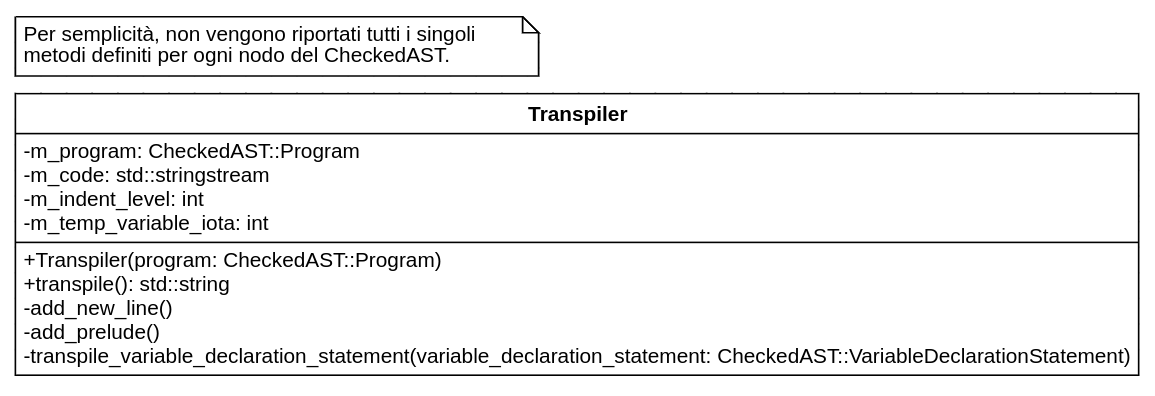
\includegraphics[width=0.9\textwidth]{figures/transpiler.png}
	\caption{Diagramma UML della classe \texttt{Transpiler}}
	\label{fig:transpiler-uml}
\end{figure}

Il \texttt{Transpiler} riceve il programma anlizzato semanticamente e genera il codice C++ con il metodo \texttt{transpile}.

Questo metodo generer\`a in ordine, le seguenti parti di codice:
\begin{itemize}
	\item \emph{prelude}, il primo frammento di codice inserito nel programma;
	\item prototipi delle funzioni, rendendo possibile la ricorsione e l'utilizzo delle funzioni prima di essere dichiarate;
	\item dichiarazioni delle funzioni;
	\item \texttt{main}, la funzione principale del programma costituita da una sola chiamata alla funzione principale del programma BugginOut rinominata in \texttt{bo\_main}.
\end{itemize}

Il \textit{prelude} \`e molto importante ed \`e costituito da:
\begin{itemize}
	\item inclusioni delle librerie necessarie per il programma;
	\item alias per i tipi primitivi, in modo da poter utilizzare i tipi di BugginOut come \texttt{i32} o \texttt{u8} senza dover scrivere \texttt{std::int32\_t} o \texttt{std::uint8\_t};
	\item definizione dei suffissi per ciascuno dei tipi primitivi, in modo da poter utilizzare i suffissi \texttt{u8}, \texttt{i32}, \texttt{f64} e \texttt{c64} per indicare i rispettivi tipi di dato in C++;
	\item definizione del tipo \texttt{bo\_range};
	\item definizione delle funzioni \textit{builtin} (\texttt{print}, \texttt{println} e \texttt{readln}).
\end{itemize}

L'approccio adottato dal \texttt{Transpiler} è di tipo \textit{top-down}, in cui la generazione del codice avviene a partire dalla radice del \texttt{CheckedAST} e si propaga ricorsivamente verso i suoi discendenti. A ciascun nodo è associato un metodo specifico, che si occupa di tradurre il costrutto corrispondente e invocare ricorsivamente i metodi per i nodi figli.

Come anticipato nella sezione \ref{sec:generazione-del-codice}, molti dei costrutti sono banali da tradurre in C++. Infatti, ad esempio:

\begin{figure}[H]
	\centering
	\begin{minted}[breaklines,frame=lines,fontsize=\footnotesize]{text}
var a = 2;
var b = 3;
var c = a + b;
	\end{minted}
	\begin{minted}[breaklines,frame=lines,fontsize=\footnotesize]{cpp}
i32 const a = (static_cast<i32>(2));
i32 const b = (static_cast<i32>(3));
i32 const c = (static_cast<i32>((a)+(b)));
	\end{minted}
	\caption{Traduzione di semplici istruzioni aritmetiche e di assegnamento}
	\label{fig:transpiler-trivial-code}
\end{figure}

Ci\`o che invece richiede pi\`u accortezza sono i tipi, le espressioni di blocco e le espressioni \texttt{if}.

Per i tipi, si eseguono le seguenti operazioni:
\begin{itemize}
	\item se il tipo \`e primitivo, si traduce direttamente in C++ grazie all'alias definito nel \textit{prelude};
	\item se il tipo \`e un puntatore, si traduce in C++ come un puntatore al tipo sottostante, perdendo, per\`o, il suo genere (\textit{weak} o \textit{strong})\footnote{Questo non ha importanza, in quanto i controlli semantici su questo sono gi\`a stati superati.};
	\item se il tipo \`e un'array, allora lo si traduce nel tipo \texttt{std::array<T, N>} con \texttt{T} tipo degli elementi e \texttt{N} dimensione dell'array;
	\item se il tipo \`e uno \textit{slice}, si traduce in C++ come un \texttt{std::span<T>} con \texttt{T} il tipo degli elementi;
	\item se il tipo \`e un \textit{range}, lo si traduce in \newline \texttt{bo\_range<ElementType, is\_inclusive>}.
\end{itemize}

Il tipo \texttt{bo\_range}, come gi\`a specificato, \`e definito nel prelude e rappresenta un intervallo di valori iterabile, parametrizzato sul tipo degli elementi (\texttt{ElementType}) e un flag booleano (\texttt{is\_inclusive}) che indica se l'estremo superiore \`e incluso o meno.

Per ci\`o che riguarda invece le espressioni di blocco e le espressioni \texttt{if}, queste vengono tradotte in C++ con un'estensione del compilatore detta \textit{compound statements}\footnote{Vedi \url{https://gcc.gnu.org/onlinedocs/gcc/Statement-Exprs.html}.}. Questa estensione \`e disponibile soo nei compilatori GNU e Clang e permette, attraverso una particolare sintassi, di restituire un valore da un blocco. Ad esempio:
\begin{figure}[H]
	\centering
	\begin{minted}[breaklines,frame=lines,fontsize=\footnotesize]{cpp}
int abs = ({
    int y = foo();
    int z;
    if (y > 0) z = y;
    else z = -y;
    z;
})
	\end{minted}
	\caption{Utilizzo di un \textit{compound statement} in C++ per calcolare il valore assoluto di \texttt{foo}}
	\label{fig:compound-statement-example}
\end{figure}

L'ulteriore componente necessaria alla loro traduzione \`e la distinzione delle espressioni di blocco in base al loro contesto di utilizzo:
\begin{itemize}
	\item se il blocco \`e il corpo di un ciclo \texttt{for} o di un'espressione \texttt{if} che non restituisce un valore, allora lo si traduce come un normale blocco ignorando l'eventuale valore restituito;
	\item se il blocco \`e il corpo di una funzione, allora lo si traduce come un normale blocco trasformando l'eventuale valore restituito in un \textit{return}.
\end{itemize}

\begin{figure}[H]
	\centering
	\begin{minted}[breaklines,frame=lines,fontsize=\footnotesize]{text}
fn foo(): i32 { 42 }
	\end{minted}
	\begin{minted}[breaklines,frame=lines,fontsize=\footnotesize]{cpp}
i32 foo()
{
    return static_cast<i32>(42);
}
	\end{minted}
	\caption{Traduzione di un'espressione di blocco utilizzato come corpo di una funzione}
	\label{fig:block-expr-as-function-body}
\end{figure}

\begin{figure}[H]
	\centering
	\begin{minted}[breaklines,frame=lines,fontsize=\footnotesize]{text}
if (a < b) {
  println("a is less than b");
} else if (a == b) {
  println("a is equal to b");
} else {
  println("a is greater than b");
}
	\end{minted}
	\begin{minted}[breaklines,frame=lines,fontsize=\footnotesize]{cpp}
if (static_cast<bool>((a)<(b)))
{
    println("a is less than b"s);
}
else
if (static_cast<bool>((a)==(b)))
{
    println("a is equal to b"s);
}
else
{
    println("a is greater than b"s);
};
	\end{minted}
	\caption{Traduzione di un'espressione di blocco utilizzata in una \texttt{if} che non restituisce alcun valore}
	\label{fig:block-expr-as-if-with-no-value}
\end{figure}

Le espressioni \texttt{if} restituenti un valore, invece, vengono tradotte come un \textit{compound statement} in cui si dichiara una variable temporanea, si traduce l'espressione \texttt{if} assegnando il valore restituito dai blocchi \textit{then} e \textit{else} a questa variabile e, alla fine del blocco, si restituisce il valore della variabile temporanea.

\`E bene notare che le espressioni \texttt{if} potrebbero essere innestate e, dunque, c'\`e bisogno che la variabile temporanea abbia sempre un nome univoco. Per fare questo si utilizza un contatore, l'attributo \texttt{m\_temp\_variable\_iota}, che viene incrementato quando si genera una nuova variabile temporanea e decrementato quando questa smette di essere visibile.

\begin{figure}[H]
	\centering
	\begin{minted}[breaklines,frame=lines,fontsize=\footnotesize]{text}
var x = if (a > b) { a } else { b };
	\end{minted}
	\begin{minted}[breaklines,frame=lines,fontsize=\footnotesize]{cpp}
i32 const x = (({
    i32 __block_ret_1 {};
    if (static_cast<bool>((a)>(b)))
    {
        __block_ret_1 = a;
    }
    else
    {
        __block_ret_1 = ({
            b;
        });
    }
    __block_ret_1;
}));
	\end{minted}
	\label{fig:if-with-value}
	\caption{Traduzione di un'espressione \texttt{if} che restituisce un valore}
\end{figure}

Una volta generato il codice C++, la stringa restituita viene memorizzata in un file con estensione \texttt{.cpp}. Questo \`e il file sorgente dato in ingresso al compilatore C++ che restituir\`a, infine, l'eseguibile del programma finale.

Il compilatore C++ utilizzato attualmente \`e \texttt{g++}, in quanto ampiamente utilizzato e, spesso, disponibile su tutti i sistemi operativi.\footnote{Di questo si parler\`a meglio nelle conclusioni.}

\section{Gestione degli errori}
\label{sec:gestione-degli-errori}

Nelle sezioni precedenti si \`e parlato di come \texttt{Lexer}, \texttt{Parser} e \texttt{Typechecker} potrebbero generare errori durante l'analisi. Volutamente, la loro gestione \`e stata omessa dai diagrammi UML, in quanto non facenti parte della logica principale di analisi. In questa sezione, si ovvia a questo, descrivendo come gli errori vengono gestiti e comunicati all'utente.

Per gli errori, si \`e scelto di non utilizzare le eccezioni di C++ in quanto queste sono poco esplicite e non permettono di avere un controllo preciso sul flusso di esecuzione del programma. Si \`e scelto quindi di seguire un approccio, in maniera a simile a quello di Rust, in cui gli errori vengono rappresentati da un tipo \texttt{Result}.

\begin{figure}[H]
	\centering
	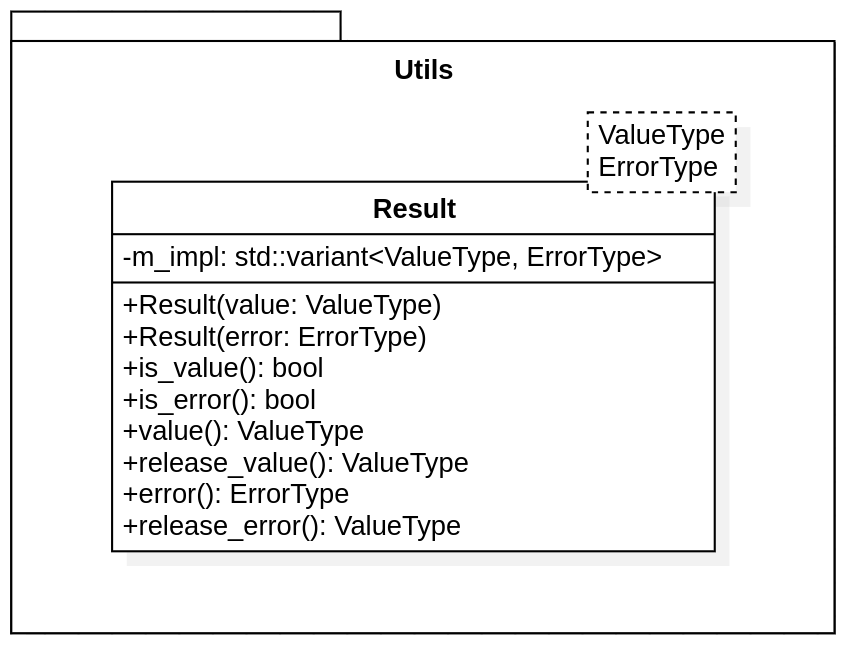
\includegraphics[width=0.7\textwidth]{figures/result.png}
	\caption{Diagramma UML del tipo \texttt{Result}}
	\label{fig:result-uml}
\end{figure}

Come possiamo vedere questo altro non \`e che un \textit{sum-type} che rappresenta un'unione disgiunta di due tipi parametrizzati: il \texttt{ValueType} e l'\texttt{ErrorType}. Il primo rappresenta il valore, senza errori, mentre il secondo rappresenta l'errore. Il tipo \texttt{Result} fornisce dei metodi per verificare se esso \`e un errore o meno, per accedere al valore o all'errore.

Per semplificare questa operazione vengono anche introdotte due \textit{macro}: \texttt{TRY} e \texttt{MUST}.

\begin{figure}[H]
	\centering
	\begin{minted}[breaklines,frame=lines,fontsize=\footnotesize]{cpp}
#define TRY(expr)                  \
  ({                               \
    auto _tmp = (expr);            \
    if (_tmp.is_error())           \
      return _tmp.release_error(); \
    _tmp.release_value();          \
  })

#define MUST(expr)           \
  ({                         \
    auto _tmp = (expr);      \
    ASSERT(_tmp.is_value()); \
    _tmp.release_value();    \
  })
	\end{minted}
	\label{fig:result-macros}
	\caption{Le \textit{macro} \texttt{TRY} e \texttt{MUST} per la gestione degli errori}
\end{figure}

La \textit{macro} \texttt{TRY} prende come parametro un espressione che restituisce un \texttt{Result} e la valuta. Se il risultato \`e un'errore allora si restiuisce l'errore e si esce dalla funzione. Altrimenti la macro restituir\`a il valore contenuto in \texttt{Result}.

La macro \texttt{MUST}, invece, fallisce se l'espressione usata come parametro restituisce un errore.

Fra le due, \texttt{TRY} \`e quella pi\`u utilizzata, in quanto permette di propagare gli errori in maniera semplice e diretta, senza dover gestire manualmente i ritorni di errore in ogni funzione. \texttt{MUST}, invece, \`e utile quando si vuole garantire che un'espressione restituisca un valore e non un errore, ad esempio quando si accede al valore di una variabile o di un'espressione che si sa essere valida.

Di seguito, si mostra un esempio di utilizzo del tipo \texttt{Result} e della \textit{macro} \texttt{TRY} per la propagazione degli errori. In questo esempio, si implementa una semplice funzione di addizione che legge due numeri interi da input e restituisce il loro risultato, gestendo gli errori di parsing e di input.

\begin{figure}[H]
	\centering
	\begin{minted}[breaklines,frame=lines,fontsize=\footnotesize]{cpp}
Result<int, std::string> parse_int(std::string_view input) {
  int value;
  auto result = std::from_chars(
    input.data(),
    input.data() + input.size(),
    value
  );

  if (result.ec != std::errc()) {
    return "Invalid integer"s;
  }

  return value;
}

Result<int, std::string> addition() {
  std::string input;

  std::getline(std::cin, input);
  if (input.empty()) {
    return "Input cannot be empty"s;
  }
  auto a = TRY(parse_int(input));

  std::getline(std::cin, input);
  if (input.empty()) {
    return "Input cannot be empty"s;
  }
  auto b = TRY(parse_int(input));

  return a + b;
}

int main() {
  auto result = addition();
  if (result.is_error()) {
    std::cerr << "Error: " << result.release_error() << std::endl;
    return 1;
  }

  std::cout << "Result: " << result.release_value() << std::endl;
  return 0;
}
	\end{minted}
	\label{fig:result-usage-example}
	\caption{Utilizzo del tipo \texttt{Result} e della \textit{macro} \texttt{TRY} per la propagazione degli errori}
\end{figure}

Nel compilatore, l'\texttt{ErrorType} utilizzato \`e proprio la classe \texttt{Error}.

\begin{figure}[H]
	\centering
	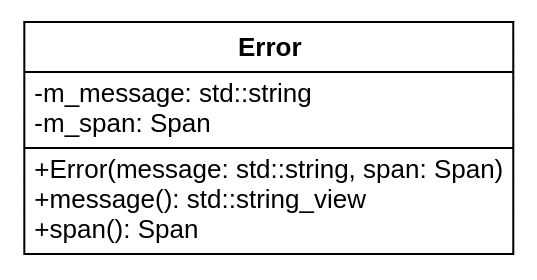
\includegraphics[width=0.6\textwidth]{figures/error.png}
	\caption{Diagramma UML della classe \texttt{Error}}
	\label{fig:error-uml}
\end{figure}

Questa contiene una semplice stringa, il messaggio d'errore, e la posizione del codice sorgente a cui l'errore fa riferimento.

Gli errori generati dalle sezioni precedenti, si propagano fino ad arrivare alla funzione principale del compilatore che li stamper\`a a schermo, come \`e stato anche visto negli esempi \ref{fig:bugginout-syntax-error}, \ref{fig:unknown-identifier-error}, \ref{fig:invalid-binary-operation-error} e \ref{fig:invalid-return-type-error}.

	% LTeX: language=it

\chapter{Alcuni esempi}
\label{chap:alcuni-esempi}

	% LTeX: language=it

\chapter*{Conclusioni}
\label{chap:conclusioni}

\section{Limiti}
\label{sec:limiti}

\section{Sviluppi futuri}
\label{sec:sviluppi-futuri}

\section{Riflessioni finali}
\label{sec:riflessioni-finali}


	\addcontentsline{toc}{chapter}{Bibliografia}
	\bibliographystyle{plain}
	\bibliography{Bibliography}
\end{document}
